\documentclass[twoside]{book}

% Packages required by doxygen
\usepackage{fixltx2e}
\usepackage{calc}
\usepackage{doxygen}
\usepackage[export]{adjustbox} % also loads graphicx
\usepackage{graphicx}
\usepackage[utf8]{inputenc}
\usepackage{makeidx}
\usepackage{multicol}
\usepackage{multirow}
\PassOptionsToPackage{warn}{textcomp}
\usepackage{textcomp}
\usepackage[nointegrals]{wasysym}
\usepackage[table]{xcolor}

% Font selection
\usepackage[T1]{fontenc}
\usepackage[scaled=.90]{helvet}
\usepackage{courier}
\usepackage{amssymb}
\usepackage{sectsty}
\renewcommand{\familydefault}{\sfdefault}
\allsectionsfont{%
  \fontseries{bc}\selectfont%
  \color{darkgray}%
}
\renewcommand{\DoxyLabelFont}{%
  \fontseries{bc}\selectfont%
  \color{darkgray}%
}
\newcommand{\+}{\discretionary{\mbox{\scriptsize$\hookleftarrow$}}{}{}}

% Page & text layout
\usepackage{geometry}
\geometry{%
  a4paper,%
  top=2.5cm,%
  bottom=2.5cm,%
  left=2.5cm,%
  right=2.5cm%
}
\tolerance=750
\hfuzz=15pt
\hbadness=750
\setlength{\emergencystretch}{15pt}
\setlength{\parindent}{0cm}
\setlength{\parskip}{0.2cm}
\makeatletter
\renewcommand{\paragraph}{%
  \@startsection{paragraph}{4}{0ex}{-1.0ex}{1.0ex}{%
    \normalfont\normalsize\bfseries\SS@parafont%
  }%
}
\renewcommand{\subparagraph}{%
  \@startsection{subparagraph}{5}{0ex}{-1.0ex}{1.0ex}{%
    \normalfont\normalsize\bfseries\SS@subparafont%
  }%
}
\makeatother

% Headers & footers
\usepackage{fancyhdr}
\pagestyle{fancyplain}
\fancyhead[LE]{\fancyplain{}{\bfseries\thepage}}
\fancyhead[CE]{\fancyplain{}{}}
\fancyhead[RE]{\fancyplain{}{\bfseries\leftmark}}
\fancyhead[LO]{\fancyplain{}{\bfseries\rightmark}}
\fancyhead[CO]{\fancyplain{}{}}
\fancyhead[RO]{\fancyplain{}{\bfseries\thepage}}
\fancyfoot[LE]{\fancyplain{}{}}
\fancyfoot[CE]{\fancyplain{}{}}
\fancyfoot[RE]{\fancyplain{}{\bfseries\scriptsize Generated by Doxygen }}
\fancyfoot[LO]{\fancyplain{}{\bfseries\scriptsize Generated by Doxygen }}
\fancyfoot[CO]{\fancyplain{}{}}
\fancyfoot[RO]{\fancyplain{}{}}
\renewcommand{\footrulewidth}{0.4pt}
\renewcommand{\chaptermark}[1]{%
  \markboth{#1}{}%
}
\renewcommand{\sectionmark}[1]{%
  \markright{\thesection\ #1}%
}

% Indices & bibliography
\usepackage{natbib}
\usepackage[titles]{tocloft}
\setcounter{tocdepth}{3}
\setcounter{secnumdepth}{5}
\makeindex

% Hyperlinks (required, but should be loaded last)
\usepackage{ifpdf}
\ifpdf
  \usepackage[pdftex,pagebackref=true]{hyperref}
\else
  \usepackage[ps2pdf,pagebackref=true]{hyperref}
\fi
\hypersetup{%
  colorlinks=true,%
  linkcolor=blue,%
  citecolor=blue,%
  unicode%
}

% Custom commands
\newcommand{\clearemptydoublepage}{%
  \newpage{\pagestyle{empty}\cleardoublepage}%
}


%===== C O N T E N T S =====

\begin{document}

% Titlepage & ToC
\hypersetup{pageanchor=false,
             bookmarks=true,
             bookmarksnumbered=true,
             pdfencoding=unicode
            }
\pagenumbering{roman}
\begin{titlepage}
\vspace*{7cm}
\begin{center}%
{\Large Software Design }\\
\vspace*{1cm}
{\large Generated by Doxygen 1.8.10}\\
\end{center}
\end{titlepage}
\clearemptydoublepage
\tableofcontents
\clearemptydoublepage
\pagenumbering{arabic}
\hypersetup{pageanchor=true}

%--- Begin generated contents ---
\chapter{Namespace Index}
\section{Namespace List}
Here is a list of all namespaces with brief descriptions\+:\begin{DoxyCompactList}
\item\contentsline{section}{\hyperlink{namespaceUi}{Ui} }{\pageref{namespaceUi}}{}
\end{DoxyCompactList}

\chapter{Hierarchical Index}
\section{Class Hierarchy}
This inheritance list is sorted roughly, but not completely, alphabetically\+:\begin{DoxyCompactList}
\item \contentsline{section}{Control\+Data}{\pageref{structControlData}}{}
\item \contentsline{section}{Machine}{\pageref{classMachine}}{}
\begin{DoxyCompactList}
\item \contentsline{section}{Movement\+Data}{\pageref{classMovementData}}{}
\end{DoxyCompactList}
\item \contentsline{section}{Socket}{\pageref{classSocket}}{}
\begin{DoxyCompactList}
\item \contentsline{section}{Server\+Socket}{\pageref{classServerSocket}}{}
\end{DoxyCompactList}
\item thread\begin{DoxyCompactList}
\item \contentsline{section}{Worker}{\pageref{classWorker}}{}
\end{DoxyCompactList}
\end{DoxyCompactList}

\chapter{Class Index}
\section{Class List}
Here are the classes, structs, unions and interfaces with brief descriptions\+:\begin{DoxyCompactList}
\item\contentsline{section}{\hyperlink{classCLIENT}{C\+L\+I\+E\+N\+T} }{\pageref{classCLIENT}}{}
\item\contentsline{section}{\hyperlink{structControlData}{Control\+Data} }{\pageref{structControlData}}{}
\item\contentsline{section}{\hyperlink{classHoymeFloors}{Hoyme\+Floors} }{\pageref{classHoymeFloors}}{}
\item\contentsline{section}{\hyperlink{classHoymeMachines}{Hoyme\+Machines} }{\pageref{classHoymeMachines}}{}
\item\contentsline{section}{\hyperlink{classHoymeMachines2}{Hoyme\+Machines2} }{\pageref{classHoymeMachines2}}{}
\item\contentsline{section}{\hyperlink{classKittFloors}{Kitt\+Floors} }{\pageref{classKittFloors}}{}
\item\contentsline{section}{\hyperlink{classMainWindow}{Main\+Window} }{\pageref{classMainWindow}}{}
\item\contentsline{section}{\hyperlink{classServerSocket}{Server\+Socket} }{\pageref{classServerSocket}}{}
\item\contentsline{section}{\hyperlink{classSocket}{Socket} }{\pageref{classSocket}}{}
\item\contentsline{section}{\hyperlink{classWorker}{Worker} }{\pageref{classWorker}}{}
\end{DoxyCompactList}

\chapter{File Index}
\section{File List}
Here is a list of all files with brief descriptions\+:\begin{DoxyCompactList}
\item\contentsline{section}{\hyperlink{client_8cpp}{client.\+cpp} }{\pageref{client_8cpp}}{}
\item\contentsline{section}{\hyperlink{PiClasses_8cpp}{Pi\+Classes.\+cpp} }{\pageref{PiClasses_8cpp}}{}
\item\contentsline{section}{\hyperlink{PiClasses_8h}{Pi\+Classes.\+h} }{\pageref{PiClasses_8h}}{}
\item\contentsline{section}{\hyperlink{pro4_8cpp}{pro4.\+cpp} }{\pageref{pro4_8cpp}}{}
\item\contentsline{section}{\hyperlink{Socket_8cpp}{Socket.\+cpp} }{\pageref{Socket_8cpp}}{}
\item\contentsline{section}{\hyperlink{Socket_8h}{Socket.\+h} }{\pageref{Socket_8h}}{}
\item\contentsline{section}{\hyperlink{Worker_8cpp}{Worker.\+cpp} }{\pageref{Worker_8cpp}}{}
\item\contentsline{section}{\hyperlink{Worker_8h}{Worker.\+h} }{\pageref{Worker_8h}}{}
\end{DoxyCompactList}

\chapter{Namespace Documentation}
\hypertarget{namespaceUi}{}\section{Ui Namespace Reference}
\label{namespaceUi}\index{Ui@{Ui}}

\chapter{Class Documentation}
\hypertarget{classCLIENT}{}\section{C\+L\+I\+E\+N\+T Class Reference}
\label{classCLIENT}\index{C\+L\+I\+E\+N\+T@{C\+L\+I\+E\+N\+T}}


{\ttfamily \#include $<$C\+L\+I\+E\+N\+T.\+h$>$}

\subsection*{Public Member Functions}
\begin{DoxyCompactItemize}
\item 
\hyperlink{classCLIENT_a75ee0d6f5c06f2fe955ce3521ae7c006}{C\+L\+I\+E\+N\+T} (string host, int port, string machine\+I\+D)
\item 
string \hyperlink{classCLIENT_a7dae67de8282043e85a51a6fce71d304}{return\+Machine\+Status} ()
\item 
string \hyperlink{classCLIENT_a4ca44e781e85e795af54eca1adc7432a}{return\+Machine\+Timer} ()
\end{DoxyCompactItemize}
\subsection*{Private Member Functions}
\begin{DoxyCompactItemize}
\item 
vector$<$ string $>$ \hyperlink{classCLIENT_a007cf416382fd529a3456f9c5db5771f}{split} (string str, char sep)
\end{DoxyCompactItemize}
\subsection*{Private Attributes}
\begin{DoxyCompactItemize}
\item 
string \hyperlink{classCLIENT_a83578b8ade6203c7a78972b3393e923b}{machine\+Status}
\item 
string \hyperlink{classCLIENT_a0474dbf26b3f3a99bf7579278453ef79}{machine\+Timer}
\item 
string \hyperlink{classCLIENT_a750c6b410d6358c35e415031dfd350c8}{connection\+Status}
\item 
bool \hyperlink{classCLIENT_af7973e9a611e41850653f69b9e9e3e8f}{cs}
\end{DoxyCompactItemize}


\subsection{Constructor \& Destructor Documentation}
\hypertarget{classCLIENT_a75ee0d6f5c06f2fe955ce3521ae7c006}{}\index{C\+L\+I\+E\+N\+T@{C\+L\+I\+E\+N\+T}!C\+L\+I\+E\+N\+T@{C\+L\+I\+E\+N\+T}}
\index{C\+L\+I\+E\+N\+T@{C\+L\+I\+E\+N\+T}!C\+L\+I\+E\+N\+T@{C\+L\+I\+E\+N\+T}}
\subsubsection[{C\+L\+I\+E\+N\+T(string host, int port, string machine\+I\+D)}]{\setlength{\rightskip}{0pt plus 5cm}C\+L\+I\+E\+N\+T\+::\+C\+L\+I\+E\+N\+T (
\begin{DoxyParamCaption}
\item[{string}]{host, }
\item[{int}]{port, }
\item[{string}]{machine\+I\+D}
\end{DoxyParamCaption}
)}\label{classCLIENT_a75ee0d6f5c06f2fe955ce3521ae7c006}

\begin{DoxyCode}
15                                                       \{
16   \hyperlink{classSocket}{Socket} sock(host.c\_str(), port);
17   \textcolor{keywordtype}{int} ret;
18 
19   \textcolor{keywordflow}{if} (sock.getConnected())\{
20     \hyperlink{classCLIENT_a750c6b410d6358c35e415031dfd350c8}{connectionStatus} = \textcolor{stringliteral}{"Conection was sucessful"};
21     \hyperlink{classCLIENT_af7973e9a611e41850653f69b9e9e3e8f}{cs} = \textcolor{keyword}{true};
22   \}
23   \textcolor{keywordflow}{else} \{
24     \hyperlink{classCLIENT_a750c6b410d6358c35e415031dfd350c8}{connectionStatus} = \textcolor{stringliteral}{"Could not connect, check your internet: socket not connected"};
25     \hyperlink{classCLIENT_a83578b8ade6203c7a78972b3393e923b}{machineStatus} = \textcolor{stringliteral}{"Connection"};
26     \hyperlink{classCLIENT_a0474dbf26b3f3a99bf7579278453ef79}{machineTimer} = \textcolor{stringliteral}{"Failed"};
27     \hyperlink{classCLIENT_af7973e9a611e41850653f69b9e9e3e8f}{cs} = \textcolor{keyword}{false};
28   \}
29 
30   \textcolor{keywordtype}{char} buff[100];
31 
32   \textcolor{keywordflow}{if} ((ret = sock.recv(buff, 100-1)) < 0) \{
33     \hyperlink{classCLIENT_a750c6b410d6358c35e415031dfd350c8}{connectionStatus} = \textcolor{stringliteral}{"Could not connect, check your internet: bad return value"};
34     \hyperlink{classCLIENT_a83578b8ade6203c7a78972b3393e923b}{machineStatus} = \textcolor{stringliteral}{"Connection"};
35     \hyperlink{classCLIENT_a0474dbf26b3f3a99bf7579278453ef79}{machineTimer} = \textcolor{stringliteral}{"Failed"};
36     cout << ret << endl;
37     \hyperlink{classCLIENT_af7973e9a611e41850653f69b9e9e3e8f}{cs} = \textcolor{keyword}{false};
38   \}
39 
40 
41 \textcolor{keywordflow}{if} (strcmp(buff, \textcolor{stringliteral}{"SVBG"}) == 0)\{      \textcolor{comment}{//happens when MAXWORKER is reached}
42         \hyperlink{classCLIENT_a83578b8ade6203c7a78972b3393e923b}{machineStatus}=\textcolor{stringliteral}{"Server"};
43         \hyperlink{classCLIENT_a0474dbf26b3f3a99bf7579278453ef79}{machineTimer}=\textcolor{stringliteral}{"Busy"};
44         \hyperlink{classCLIENT_af7973e9a611e41850653f69b9e9e3e8f}{cs}=\textcolor{keyword}{false};
45       \}
46   cout << \hyperlink{classCLIENT_a750c6b410d6358c35e415031dfd350c8}{connectionStatus} << endl;
47   \textcolor{comment}{// assert:  welcome message received and connection to server completed}
48 
49   \textcolor{keywordflow}{while} (\hyperlink{classCLIENT_af7973e9a611e41850653f69b9e9e3e8f}{cs}) \{
50     sock.send(machineID.c\_str(), machineID.size());
51     ret = sock.recv(buff, 100-1);
52     buff[ret] = \textcolor{charliteral}{'\(\backslash\)0'};  \textcolor{comment}{// add terminating nullbyte to received array of char}
53     cout<<ret;
54     \textcolor{keywordtype}{string} information = buff;
55     cout << buff << endl;
56     vector<string> parts = \hyperlink{classCLIENT_a007cf416382fd529a3456f9c5db5771f}{split}(information, \textcolor{charliteral}{'-'});
57 
58 
59     \textcolor{keywordflow}{if}(ret == 0)\{
60         \hyperlink{classCLIENT_a83578b8ade6203c7a78972b3393e923b}{machineStatus} = \textcolor{stringliteral}{"Data not"};
61         \hyperlink{classCLIENT_a0474dbf26b3f3a99bf7579278453ef79}{machineTimer} = \textcolor{stringliteral}{"received"};
62     \}
63 
64     \textcolor{keywordflow}{else} \textcolor{keywordflow}{if} (strcmp(buff, \textcolor{stringliteral}{"EPIC"}) == 0)\{   \textcolor{comment}{//happens when status.dat isn't found}
65       \hyperlink{classCLIENT_a83578b8ade6203c7a78972b3393e923b}{machineStatus}=\textcolor{stringliteral}{"Pi Configuration"};
66       \hyperlink{classCLIENT_a0474dbf26b3f3a99bf7579278453ef79}{machineTimer}=\textcolor{stringliteral}{"Error"};
67     \}
68 
69  \textcolor{comment}{/*   else if (strcmp(buff, "SVBG") == 0)\{      //happens when MAXWORKER is reached}
70 \textcolor{comment}{      machineStatus="Server";}
71 \textcolor{comment}{      machineTimer="Busy";}
72 \textcolor{comment}{      sock.close();}
73 \textcolor{comment}{      break;}
74 \textcolor{comment}{    \}*/}
75 
76     \textcolor{keywordflow}{else} \textcolor{keywordflow}{if} (strcmp(buff, \textcolor{stringliteral}{"NSFD"}) == 0)\{      \textcolor{comment}{//happens when dev/ttyACMx isn't found by Pi}
77 
78       \hyperlink{classCLIENT_a83578b8ade6203c7a78972b3393e923b}{machineStatus}=\textcolor{stringliteral}{"Sensor"};
79       \hyperlink{classCLIENT_a0474dbf26b3f3a99bf7579278453ef79}{machineTimer}=\textcolor{stringliteral}{"Not Found"};
80     \}
81 
82     \textcolor{keywordflow}{else} \textcolor{keywordflow}{if} (strcmp(buff, \textcolor{stringliteral}{"WRCD"}) == 0)\{          \textcolor{comment}{//happend when wrong machine Id is sent to Pi}
83       \hyperlink{classCLIENT_a83578b8ade6203c7a78972b3393e923b}{machineStatus}=\textcolor{stringliteral}{"Configuration"};
84       \hyperlink{classCLIENT_a0474dbf26b3f3a99bf7579278453ef79}{machineTimer}=\textcolor{stringliteral}{"Error"};
85     \}
86 
87     \textcolor{keywordflow}{else} \textcolor{keywordflow}{if} (information == \textcolor{stringliteral}{"DONE"}) \{
88         sock.send(\textcolor{stringliteral}{"END"}, 3);
89         sock.close();
90         \textcolor{keywordflow}{break};
91       \}
92 
93 
94      \textcolor{keywordflow}{else} \textcolor{keywordflow}{if} (parts.size() != 2) \{
95           cerr << \textcolor{stringliteral}{"invalid data"} << endl;
96           cerr << \textcolor{stringliteral}{"recieved string: "} << information << endl;
97           \hyperlink{classCLIENT_a83578b8ade6203c7a78972b3393e923b}{machineStatus}=\textcolor{stringliteral}{"Invalid"};
98           \hyperlink{classCLIENT_a0474dbf26b3f3a99bf7579278453ef79}{machineTimer}= \textcolor{stringliteral}{"Response"};
99     \}
100 
101 
102     \textcolor{keywordflow}{else}\{
103          \hyperlink{classCLIENT_a83578b8ade6203c7a78972b3393e923b}{machineStatus} = parts.at(0);
104          \hyperlink{classCLIENT_a0474dbf26b3f3a99bf7579278453ef79}{machineTimer} = parts.at(1);
105     \}
106 
107 
108     sock.send(\textcolor{stringliteral}{"DONE"}, 4);
109 
110     \textcolor{keywordflow}{if} (information == \textcolor{stringliteral}{"DONE"}) \{
111       sock.send(\textcolor{stringliteral}{"END"}, 3);
112       sock.close();
113       \textcolor{keywordflow}{break};
114     \}
115   \}
116 \}
\end{DoxyCode}


\subsection{Member Function Documentation}
\hypertarget{classCLIENT_a7dae67de8282043e85a51a6fce71d304}{}\index{C\+L\+I\+E\+N\+T@{C\+L\+I\+E\+N\+T}!return\+Machine\+Status@{return\+Machine\+Status}}
\index{return\+Machine\+Status@{return\+Machine\+Status}!C\+L\+I\+E\+N\+T@{C\+L\+I\+E\+N\+T}}
\subsubsection[{return\+Machine\+Status()}]{\setlength{\rightskip}{0pt plus 5cm}string C\+L\+I\+E\+N\+T\+::return\+Machine\+Status (
\begin{DoxyParamCaption}
{}
\end{DoxyParamCaption}
)}\label{classCLIENT_a7dae67de8282043e85a51a6fce71d304}

\begin{DoxyCode}
131                                   \{
132   \textcolor{keywordflow}{return} \hyperlink{classCLIENT_a83578b8ade6203c7a78972b3393e923b}{machineStatus};
133 \}
\end{DoxyCode}
\hypertarget{classCLIENT_a4ca44e781e85e795af54eca1adc7432a}{}\index{C\+L\+I\+E\+N\+T@{C\+L\+I\+E\+N\+T}!return\+Machine\+Timer@{return\+Machine\+Timer}}
\index{return\+Machine\+Timer@{return\+Machine\+Timer}!C\+L\+I\+E\+N\+T@{C\+L\+I\+E\+N\+T}}
\subsubsection[{return\+Machine\+Timer()}]{\setlength{\rightskip}{0pt plus 5cm}string C\+L\+I\+E\+N\+T\+::return\+Machine\+Timer (
\begin{DoxyParamCaption}
{}
\end{DoxyParamCaption}
)}\label{classCLIENT_a4ca44e781e85e795af54eca1adc7432a}

\begin{DoxyCode}
135                                  \{
136   \textcolor{keywordflow}{return} \hyperlink{classCLIENT_a0474dbf26b3f3a99bf7579278453ef79}{machineTimer};
137 \}
\end{DoxyCode}
\hypertarget{classCLIENT_a007cf416382fd529a3456f9c5db5771f}{}\index{C\+L\+I\+E\+N\+T@{C\+L\+I\+E\+N\+T}!split@{split}}
\index{split@{split}!C\+L\+I\+E\+N\+T@{C\+L\+I\+E\+N\+T}}
\subsubsection[{split(string str, char sep)}]{\setlength{\rightskip}{0pt plus 5cm}vector$<$ string $>$ C\+L\+I\+E\+N\+T\+::split (
\begin{DoxyParamCaption}
\item[{string}]{str, }
\item[{char}]{sep}
\end{DoxyParamCaption}
)\hspace{0.3cm}{\ttfamily [private]}}\label{classCLIENT_a007cf416382fd529a3456f9c5db5771f}

\begin{DoxyCode}
118                                                  \{
119   stringstream test(str);
120   \textcolor{keywordtype}{string} segment;
121   vector<string> seglist;
122 
123   \textcolor{keywordflow}{while}(getline(test, segment, sep)) \{
124    seglist.push\_back(segment);
125   \}
126 
127   \textcolor{keywordflow}{return} seglist;
128 \}
\end{DoxyCode}


\subsection{Member Data Documentation}
\hypertarget{classCLIENT_a750c6b410d6358c35e415031dfd350c8}{}\index{C\+L\+I\+E\+N\+T@{C\+L\+I\+E\+N\+T}!connection\+Status@{connection\+Status}}
\index{connection\+Status@{connection\+Status}!C\+L\+I\+E\+N\+T@{C\+L\+I\+E\+N\+T}}
\subsubsection[{connection\+Status}]{\setlength{\rightskip}{0pt plus 5cm}string C\+L\+I\+E\+N\+T\+::connection\+Status\hspace{0.3cm}{\ttfamily [private]}}\label{classCLIENT_a750c6b410d6358c35e415031dfd350c8}
\hypertarget{classCLIENT_af7973e9a611e41850653f69b9e9e3e8f}{}\index{C\+L\+I\+E\+N\+T@{C\+L\+I\+E\+N\+T}!cs@{cs}}
\index{cs@{cs}!C\+L\+I\+E\+N\+T@{C\+L\+I\+E\+N\+T}}
\subsubsection[{cs}]{\setlength{\rightskip}{0pt plus 5cm}bool C\+L\+I\+E\+N\+T\+::cs\hspace{0.3cm}{\ttfamily [private]}}\label{classCLIENT_af7973e9a611e41850653f69b9e9e3e8f}
\hypertarget{classCLIENT_a83578b8ade6203c7a78972b3393e923b}{}\index{C\+L\+I\+E\+N\+T@{C\+L\+I\+E\+N\+T}!machine\+Status@{machine\+Status}}
\index{machine\+Status@{machine\+Status}!C\+L\+I\+E\+N\+T@{C\+L\+I\+E\+N\+T}}
\subsubsection[{machine\+Status}]{\setlength{\rightskip}{0pt plus 5cm}string C\+L\+I\+E\+N\+T\+::machine\+Status\hspace{0.3cm}{\ttfamily [private]}}\label{classCLIENT_a83578b8ade6203c7a78972b3393e923b}
\hypertarget{classCLIENT_a0474dbf26b3f3a99bf7579278453ef79}{}\index{C\+L\+I\+E\+N\+T@{C\+L\+I\+E\+N\+T}!machine\+Timer@{machine\+Timer}}
\index{machine\+Timer@{machine\+Timer}!C\+L\+I\+E\+N\+T@{C\+L\+I\+E\+N\+T}}
\subsubsection[{machine\+Timer}]{\setlength{\rightskip}{0pt plus 5cm}string C\+L\+I\+E\+N\+T\+::machine\+Timer\hspace{0.3cm}{\ttfamily [private]}}\label{classCLIENT_a0474dbf26b3f3a99bf7579278453ef79}


The documentation for this class was generated from the following files\+:\begin{DoxyCompactItemize}
\item 
\hyperlink{CLIENT_8h}{C\+L\+I\+E\+N\+T.\+h}\item 
\hyperlink{CLIENT_8cpp}{C\+L\+I\+E\+N\+T.\+cpp}\item 
\hyperlink{CLIENT1_8cpp}{C\+L\+I\+E\+N\+T1.\+cpp}\item 
\hyperlink{CLIENT2_8cpp}{C\+L\+I\+E\+N\+T2.\+cpp}\end{DoxyCompactItemize}

\hypertarget{structControlData}{}\section{Control\+Data Struct Reference}
\label{structControlData}\index{Control\+Data@{Control\+Data}}


{\ttfamily \#include $<$Worker.\+h$>$}

\subsection*{Public Member Functions}
\begin{DoxyCompactItemize}
\item 
\hyperlink{structControlData_a575219e5e0bc27904dc2aa7b1315d356}{Control\+Data} ()
\end{DoxyCompactItemize}
\subsection*{Public Attributes}
\begin{DoxyCompactItemize}
\item 
atomic$<$ int $>$ \hyperlink{structControlData_ac8fbf80345423cf5650ae64bfb10dc88}{contin}
\end{DoxyCompactItemize}


\subsection{Detailed Description}
data structure for managing control of the server 

\subsection{Constructor \& Destructor Documentation}
\hypertarget{structControlData_a575219e5e0bc27904dc2aa7b1315d356}{}\index{Control\+Data@{Control\+Data}!Control\+Data@{Control\+Data}}
\index{Control\+Data@{Control\+Data}!Control\+Data@{Control\+Data}}
\subsubsection[{Control\+Data()}]{\setlength{\rightskip}{0pt plus 5cm}Control\+Data\+::\+Control\+Data (
\begin{DoxyParamCaption}
{}
\end{DoxyParamCaption}
)\hspace{0.3cm}{\ttfamily [inline]}}\label{structControlData_a575219e5e0bc27904dc2aa7b1315d356}
default constructor \begin{DoxyParagraph}{State Changes}
assign 1 to contin 
\end{DoxyParagraph}

\begin{DoxyCode}
19 \{ \hyperlink{structControlData_ac8fbf80345423cf5650ae64bfb10dc88}{contin} = 1; \}
\end{DoxyCode}


\subsection{Member Data Documentation}
\hypertarget{structControlData_ac8fbf80345423cf5650ae64bfb10dc88}{}\index{Control\+Data@{Control\+Data}!contin@{contin}}
\index{contin@{contin}!Control\+Data@{Control\+Data}}
\subsubsection[{contin}]{\setlength{\rightskip}{0pt plus 5cm}atomic$<$int$>$ Control\+Data\+::contin}\label{structControlData_ac8fbf80345423cf5650ae64bfb10dc88}
continue serving while contin is non-\/zero. The type atomic$<$int$>$ prevents \char`\"{}race condition\char`\"{} errors if multiple threads try to access contin at the same time 

The documentation for this struct was generated from the following file\+:\begin{DoxyCompactItemize}
\item 
\hyperlink{Worker_8h}{Worker.\+h}\end{DoxyCompactItemize}

\hypertarget{classHoymeFloors}{}\section{Hoyme\+Floors Class Reference}
\label{classHoymeFloors}\index{Hoyme\+Floors@{Hoyme\+Floors}}


{\ttfamily \#include $<$hoymefloors.\+h$>$}

Inheritance diagram for Hoyme\+Floors\+:\begin{figure}[H]
\begin{center}
\leavevmode
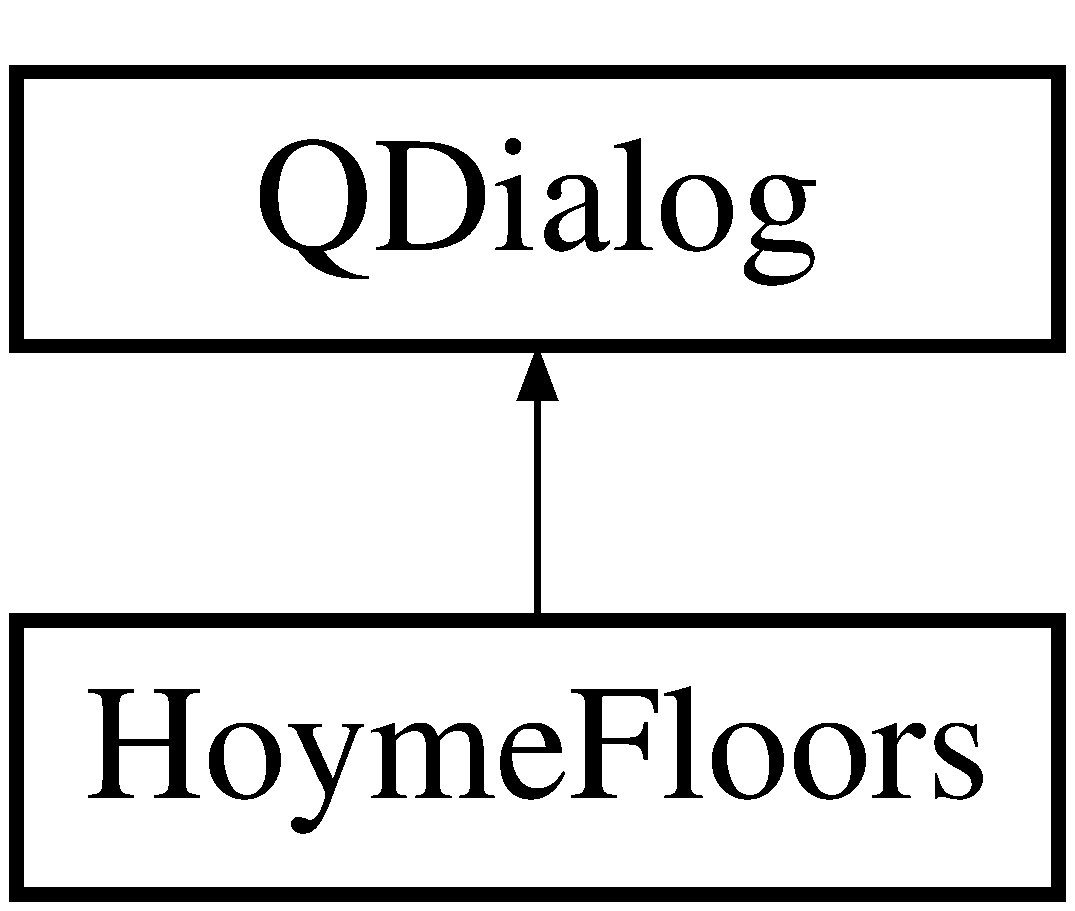
\includegraphics[height=2.000000cm]{classHoymeFloors}
\end{center}
\end{figure}
\subsection*{Public Member Functions}
\begin{DoxyCompactItemize}
\item 
\hyperlink{classHoymeFloors_a708e4152c6f1de58b3d4c2b8cd1a2cac}{Hoyme\+Floors} (Q\+Widget $\ast$parent=0)
\item 
\hyperlink{classHoymeFloors_a22b8863dcc7cabf61e3a5f6221f9fc69}{$\sim$\+Hoyme\+Floors} ()
\end{DoxyCompactItemize}
\subsection*{Private Slots}
\begin{DoxyCompactItemize}
\item 
void \hyperlink{classHoymeFloors_ab07d53faecc2b6d9afa20ce673bbfeb8}{on\+\_\+push\+Button\+\_\+clicked} ()
\item 
void \hyperlink{classHoymeFloors_a2c34701acc5383216634845ee813dcf9}{on\+\_\+push\+Button\+\_\+2\+\_\+clicked} ()
\end{DoxyCompactItemize}
\subsection*{Private Attributes}
\begin{DoxyCompactItemize}
\item 
Ui\+::\+Hoyme\+Floors $\ast$ \hyperlink{classHoymeFloors_ade5233dfacee00a835b2be807e2ec239}{ui}
\end{DoxyCompactItemize}


\subsection{Constructor \& Destructor Documentation}
\hypertarget{classHoymeFloors_a708e4152c6f1de58b3d4c2b8cd1a2cac}{}\index{Hoyme\+Floors@{Hoyme\+Floors}!Hoyme\+Floors@{Hoyme\+Floors}}
\index{Hoyme\+Floors@{Hoyme\+Floors}!Hoyme\+Floors@{Hoyme\+Floors}}
\subsubsection[{Hoyme\+Floors(\+Q\+Widget $\ast$parent=0)}]{\setlength{\rightskip}{0pt plus 5cm}Hoyme\+Floors\+::\+Hoyme\+Floors (
\begin{DoxyParamCaption}
\item[{Q\+Widget $\ast$}]{parent = {\ttfamily 0}}
\end{DoxyParamCaption}
)\hspace{0.3cm}{\ttfamily [explicit]}}\label{classHoymeFloors_a708e4152c6f1de58b3d4c2b8cd1a2cac}

\begin{DoxyCode}
6                                         :
7     QDialog(parent),
8     \hyperlink{classHoymeFloors_ade5233dfacee00a835b2be807e2ec239}{ui}(\textcolor{keyword}{new} Ui::HoymeFloors)
9 \{
10     \hyperlink{classHoymeFloors_ade5233dfacee00a835b2be807e2ec239}{ui}->setupUi(\textcolor{keyword}{this});
11 \}
\end{DoxyCode}
\hypertarget{classHoymeFloors_a22b8863dcc7cabf61e3a5f6221f9fc69}{}\index{Hoyme\+Floors@{Hoyme\+Floors}!````~Hoyme\+Floors@{$\sim$\+Hoyme\+Floors}}
\index{````~Hoyme\+Floors@{$\sim$\+Hoyme\+Floors}!Hoyme\+Floors@{Hoyme\+Floors}}
\subsubsection[{$\sim$\+Hoyme\+Floors()}]{\setlength{\rightskip}{0pt plus 5cm}Hoyme\+Floors\+::$\sim$\+Hoyme\+Floors (
\begin{DoxyParamCaption}
{}
\end{DoxyParamCaption}
)}\label{classHoymeFloors_a22b8863dcc7cabf61e3a5f6221f9fc69}

\begin{DoxyCode}
14 \{
15     \textcolor{keyword}{delete} \hyperlink{classHoymeFloors_ade5233dfacee00a835b2be807e2ec239}{ui};
16 \}
\end{DoxyCode}


\subsection{Member Function Documentation}
\hypertarget{classHoymeFloors_a2c34701acc5383216634845ee813dcf9}{}\index{Hoyme\+Floors@{Hoyme\+Floors}!on\+\_\+push\+Button\+\_\+2\+\_\+clicked@{on\+\_\+push\+Button\+\_\+2\+\_\+clicked}}
\index{on\+\_\+push\+Button\+\_\+2\+\_\+clicked@{on\+\_\+push\+Button\+\_\+2\+\_\+clicked}!Hoyme\+Floors@{Hoyme\+Floors}}
\subsubsection[{on\+\_\+push\+Button\+\_\+2\+\_\+clicked}]{\setlength{\rightskip}{0pt plus 5cm}void Hoyme\+Floors\+::on\+\_\+push\+Button\+\_\+2\+\_\+clicked (
\begin{DoxyParamCaption}
{}
\end{DoxyParamCaption}
)\hspace{0.3cm}{\ttfamily [private]}, {\ttfamily [slot]}}\label{classHoymeFloors_a2c34701acc5383216634845ee813dcf9}

\begin{DoxyCode}
26 \{
27     \hyperlink{classHoymeMachines2}{HoymeMachines2} hMch2;
28     hMch2.setModal(\textcolor{keyword}{true});
29     hMch2.exec();
30 \}
\end{DoxyCode}
\hypertarget{classHoymeFloors_ab07d53faecc2b6d9afa20ce673bbfeb8}{}\index{Hoyme\+Floors@{Hoyme\+Floors}!on\+\_\+push\+Button\+\_\+clicked@{on\+\_\+push\+Button\+\_\+clicked}}
\index{on\+\_\+push\+Button\+\_\+clicked@{on\+\_\+push\+Button\+\_\+clicked}!Hoyme\+Floors@{Hoyme\+Floors}}
\subsubsection[{on\+\_\+push\+Button\+\_\+clicked}]{\setlength{\rightskip}{0pt plus 5cm}void Hoyme\+Floors\+::on\+\_\+push\+Button\+\_\+clicked (
\begin{DoxyParamCaption}
{}
\end{DoxyParamCaption}
)\hspace{0.3cm}{\ttfamily [private]}, {\ttfamily [slot]}}\label{classHoymeFloors_ab07d53faecc2b6d9afa20ce673bbfeb8}

\begin{DoxyCode}
19 \{
20     \hyperlink{classHoymeMachines}{HoymeMachines} hMch;
21     hMch.setModal(\textcolor{keyword}{true});
22     hMch.exec();
23 \}
\end{DoxyCode}


\subsection{Member Data Documentation}
\hypertarget{classHoymeFloors_ade5233dfacee00a835b2be807e2ec239}{}\index{Hoyme\+Floors@{Hoyme\+Floors}!ui@{ui}}
\index{ui@{ui}!Hoyme\+Floors@{Hoyme\+Floors}}
\subsubsection[{ui}]{\setlength{\rightskip}{0pt plus 5cm}Ui\+::\+Hoyme\+Floors$\ast$ Hoyme\+Floors\+::ui\hspace{0.3cm}{\ttfamily [private]}}\label{classHoymeFloors_ade5233dfacee00a835b2be807e2ec239}


The documentation for this class was generated from the following files\+:\begin{DoxyCompactItemize}
\item 
\hyperlink{hoymefloors_8h}{hoymefloors.\+h}\item 
\hyperlink{hoymefloors_8cpp}{hoymefloors.\+cpp}\end{DoxyCompactItemize}

\hypertarget{classHoymeMachines}{}\section{Hoyme\+Machines Class Reference}
\label{classHoymeMachines}\index{Hoyme\+Machines@{Hoyme\+Machines}}


{\ttfamily \#include $<$hoymemachines.\+h$>$}

Inheritance diagram for Hoyme\+Machines\+:\begin{figure}[H]
\begin{center}
\leavevmode
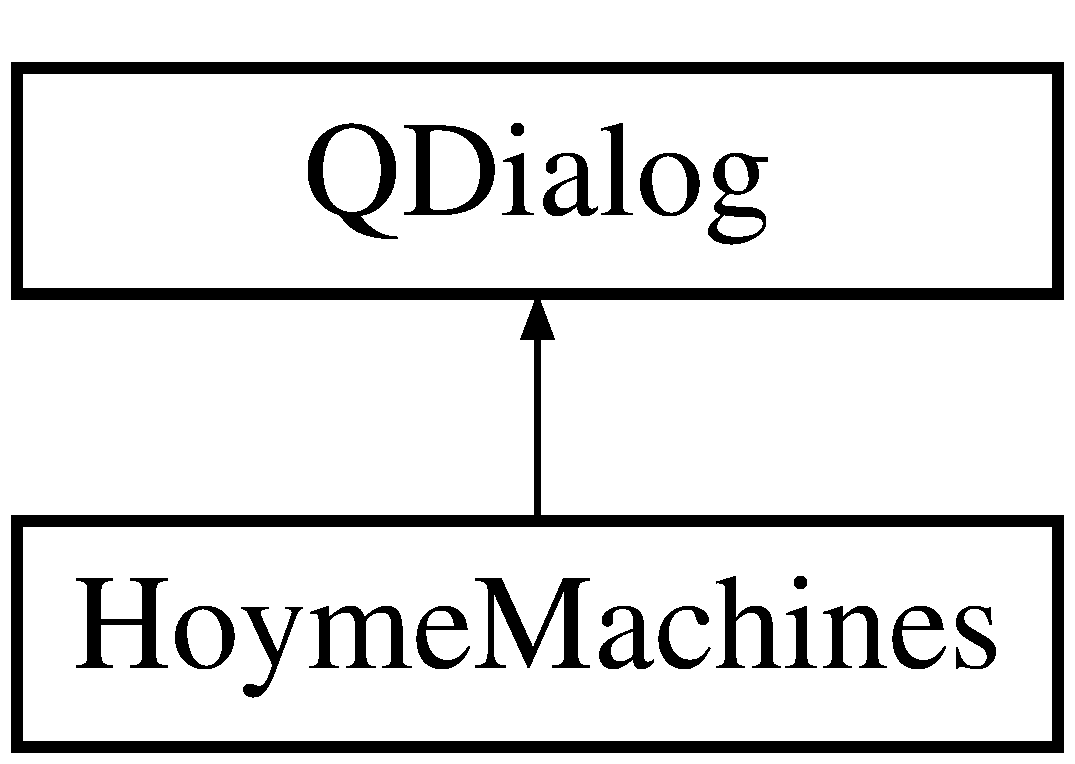
\includegraphics[height=2.000000cm]{classHoymeMachines}
\end{center}
\end{figure}
\subsection*{Public Member Functions}
\begin{DoxyCompactItemize}
\item 
\hyperlink{classHoymeMachines_af118b420693258a5a4ec10810f02a7ec}{Hoyme\+Machines} (Q\+Widget $\ast$parent=0)
\item 
\hyperlink{classHoymeMachines_a6aa418fc62c58137171e313c1ace4ccf}{$\sim$\+Hoyme\+Machines} ()
\end{DoxyCompactItemize}
\subsection*{Private Slots}
\begin{DoxyCompactItemize}
\item 
void \hyperlink{classHoymeMachines_a34b497f41441b0dd94fc0181798daa92}{on\+\_\+push\+Button\+\_\+clicked} ()
\item 
void \hyperlink{classHoymeMachines_ae6dbb429a5f917a656d34f42de4f32fe}{on\+\_\+push\+Button\+\_\+2\+\_\+clicked} ()
\item 
void \hyperlink{classHoymeMachines_a884d8539f9bdeb71acbe4a7381114f42}{on\+\_\+push\+Button\+\_\+3\+\_\+clicked} ()
\end{DoxyCompactItemize}
\subsection*{Private Attributes}
\begin{DoxyCompactItemize}
\item 
Ui\+::\+Hoyme\+Machines $\ast$ \hyperlink{classHoymeMachines_a72f3067484ba8b1cfa5dbb5e1b7025ba}{ui}
\end{DoxyCompactItemize}


\subsection{Constructor \& Destructor Documentation}
\hypertarget{classHoymeMachines_af118b420693258a5a4ec10810f02a7ec}{}\index{Hoyme\+Machines@{Hoyme\+Machines}!Hoyme\+Machines@{Hoyme\+Machines}}
\index{Hoyme\+Machines@{Hoyme\+Machines}!Hoyme\+Machines@{Hoyme\+Machines}}
\subsubsection[{Hoyme\+Machines(\+Q\+Widget $\ast$parent=0)}]{\setlength{\rightskip}{0pt plus 5cm}Hoyme\+Machines\+::\+Hoyme\+Machines (
\begin{DoxyParamCaption}
\item[{Q\+Widget $\ast$}]{parent = {\ttfamily 0}}
\end{DoxyParamCaption}
)\hspace{0.3cm}{\ttfamily [explicit]}}\label{classHoymeMachines_af118b420693258a5a4ec10810f02a7ec}

\begin{DoxyCode}
16                                             :
17     QDialog(parent),
18     \hyperlink{classHoymeMachines_a72f3067484ba8b1cfa5dbb5e1b7025ba}{ui}(\textcolor{keyword}{new} Ui::HoymeMachines)
19 \{
20     \hyperlink{classHoymeMachines_a72f3067484ba8b1cfa5dbb5e1b7025ba}{ui}->setupUi(\textcolor{keyword}{this});
21 \}
\end{DoxyCode}
\hypertarget{classHoymeMachines_a6aa418fc62c58137171e313c1ace4ccf}{}\index{Hoyme\+Machines@{Hoyme\+Machines}!````~Hoyme\+Machines@{$\sim$\+Hoyme\+Machines}}
\index{````~Hoyme\+Machines@{$\sim$\+Hoyme\+Machines}!Hoyme\+Machines@{Hoyme\+Machines}}
\subsubsection[{$\sim$\+Hoyme\+Machines()}]{\setlength{\rightskip}{0pt plus 5cm}Hoyme\+Machines\+::$\sim$\+Hoyme\+Machines (
\begin{DoxyParamCaption}
{}
\end{DoxyParamCaption}
)}\label{classHoymeMachines_a6aa418fc62c58137171e313c1ace4ccf}

\begin{DoxyCode}
24 \{
25     \textcolor{keyword}{delete} \hyperlink{classHoymeMachines_a72f3067484ba8b1cfa5dbb5e1b7025ba}{ui};
26 \}
\end{DoxyCode}


\subsection{Member Function Documentation}
\hypertarget{classHoymeMachines_ae6dbb429a5f917a656d34f42de4f32fe}{}\index{Hoyme\+Machines@{Hoyme\+Machines}!on\+\_\+push\+Button\+\_\+2\+\_\+clicked@{on\+\_\+push\+Button\+\_\+2\+\_\+clicked}}
\index{on\+\_\+push\+Button\+\_\+2\+\_\+clicked@{on\+\_\+push\+Button\+\_\+2\+\_\+clicked}!Hoyme\+Machines@{Hoyme\+Machines}}
\subsubsection[{on\+\_\+push\+Button\+\_\+2\+\_\+clicked}]{\setlength{\rightskip}{0pt plus 5cm}void Hoyme\+Machines\+::on\+\_\+push\+Button\+\_\+2\+\_\+clicked (
\begin{DoxyParamCaption}
{}
\end{DoxyParamCaption}
)\hspace{0.3cm}{\ttfamily [private]}, {\ttfamily [slot]}}\label{classHoymeMachines_ae6dbb429a5f917a656d34f42de4f32fe}

\begin{DoxyCode}
38 \{
39     \hyperlink{classCLIENT}{CLIENT} client2 (\textcolor{stringliteral}{"rns202-13.cs.stolaf.edu"},25274, \textcolor{stringliteral}{"hmh-01-124-l"} );
40     \hyperlink{classHoymeMachines_a72f3067484ba8b1cfa5dbb5e1b7025ba}{ui}->label\_2->setText(QString(client2.returnMachineStatus().c\_str()));
41     \hyperlink{classHoymeMachines_a72f3067484ba8b1cfa5dbb5e1b7025ba}{ui}->label\_5->setText(QString(client2.returnMachineTimer().c\_str()));
42 \}
\end{DoxyCode}
\hypertarget{classHoymeMachines_a884d8539f9bdeb71acbe4a7381114f42}{}\index{Hoyme\+Machines@{Hoyme\+Machines}!on\+\_\+push\+Button\+\_\+3\+\_\+clicked@{on\+\_\+push\+Button\+\_\+3\+\_\+clicked}}
\index{on\+\_\+push\+Button\+\_\+3\+\_\+clicked@{on\+\_\+push\+Button\+\_\+3\+\_\+clicked}!Hoyme\+Machines@{Hoyme\+Machines}}
\subsubsection[{on\+\_\+push\+Button\+\_\+3\+\_\+clicked}]{\setlength{\rightskip}{0pt plus 5cm}void Hoyme\+Machines\+::on\+\_\+push\+Button\+\_\+3\+\_\+clicked (
\begin{DoxyParamCaption}
{}
\end{DoxyParamCaption}
)\hspace{0.3cm}{\ttfamily [private]}, {\ttfamily [slot]}}\label{classHoymeMachines_a884d8539f9bdeb71acbe4a7381114f42}

\begin{DoxyCode}
46 \{
47     \hyperlink{classHoymeMachines_a72f3067484ba8b1cfa5dbb5e1b7025ba}{ui}->label\_3->setText(\textcolor{stringliteral}{"Open"});
48     \hyperlink{classHoymeMachines_a72f3067484ba8b1cfa5dbb5e1b7025ba}{ui}->label\_6->setText(\textcolor{stringliteral}{"0 minutes"});
49 \}
\end{DoxyCode}
\hypertarget{classHoymeMachines_a34b497f41441b0dd94fc0181798daa92}{}\index{Hoyme\+Machines@{Hoyme\+Machines}!on\+\_\+push\+Button\+\_\+clicked@{on\+\_\+push\+Button\+\_\+clicked}}
\index{on\+\_\+push\+Button\+\_\+clicked@{on\+\_\+push\+Button\+\_\+clicked}!Hoyme\+Machines@{Hoyme\+Machines}}
\subsubsection[{on\+\_\+push\+Button\+\_\+clicked}]{\setlength{\rightskip}{0pt plus 5cm}void Hoyme\+Machines\+::on\+\_\+push\+Button\+\_\+clicked (
\begin{DoxyParamCaption}
{}
\end{DoxyParamCaption}
)\hspace{0.3cm}{\ttfamily [private]}, {\ttfamily [slot]}}\label{classHoymeMachines_a34b497f41441b0dd94fc0181798daa92}

\begin{DoxyCode}
31 \{
32     \hyperlink{classCLIENT}{CLIENT} client1 (\textcolor{stringliteral}{"130.71.214.164"},25279, \textcolor{stringliteral}{"hmh-02-123-l"} );                       \textcolor{comment}{//make sure that
       the ip address is right and that there is a server running with this socket number}
33     \hyperlink{classHoymeMachines_a72f3067484ba8b1cfa5dbb5e1b7025ba}{ui}->washer\_1\_status->setText(QString(client1.returnMachineStatus().c\_str()));
34     \hyperlink{classHoymeMachines_a72f3067484ba8b1cfa5dbb5e1b7025ba}{ui}->washer\_1\_timer->setText(QString(client1.returnMachineTimer().c\_str()));
35 \}
\end{DoxyCode}


\subsection{Member Data Documentation}
\hypertarget{classHoymeMachines_a72f3067484ba8b1cfa5dbb5e1b7025ba}{}\index{Hoyme\+Machines@{Hoyme\+Machines}!ui@{ui}}
\index{ui@{ui}!Hoyme\+Machines@{Hoyme\+Machines}}
\subsubsection[{ui}]{\setlength{\rightskip}{0pt plus 5cm}Ui\+::\+Hoyme\+Machines$\ast$ Hoyme\+Machines\+::ui\hspace{0.3cm}{\ttfamily [private]}}\label{classHoymeMachines_a72f3067484ba8b1cfa5dbb5e1b7025ba}


The documentation for this class was generated from the following files\+:\begin{DoxyCompactItemize}
\item 
\hyperlink{hoymemachines_8h}{hoymemachines.\+h}\item 
\hyperlink{hoymemachines_8cpp}{hoymemachines.\+cpp}\end{DoxyCompactItemize}

\hypertarget{classHoymeMachines2}{}\section{Hoyme\+Machines2 Class Reference}
\label{classHoymeMachines2}\index{Hoyme\+Machines2@{Hoyme\+Machines2}}


{\ttfamily \#include $<$hoymemachines2.\+h$>$}

Inheritance diagram for Hoyme\+Machines2\+:\begin{figure}[H]
\begin{center}
\leavevmode
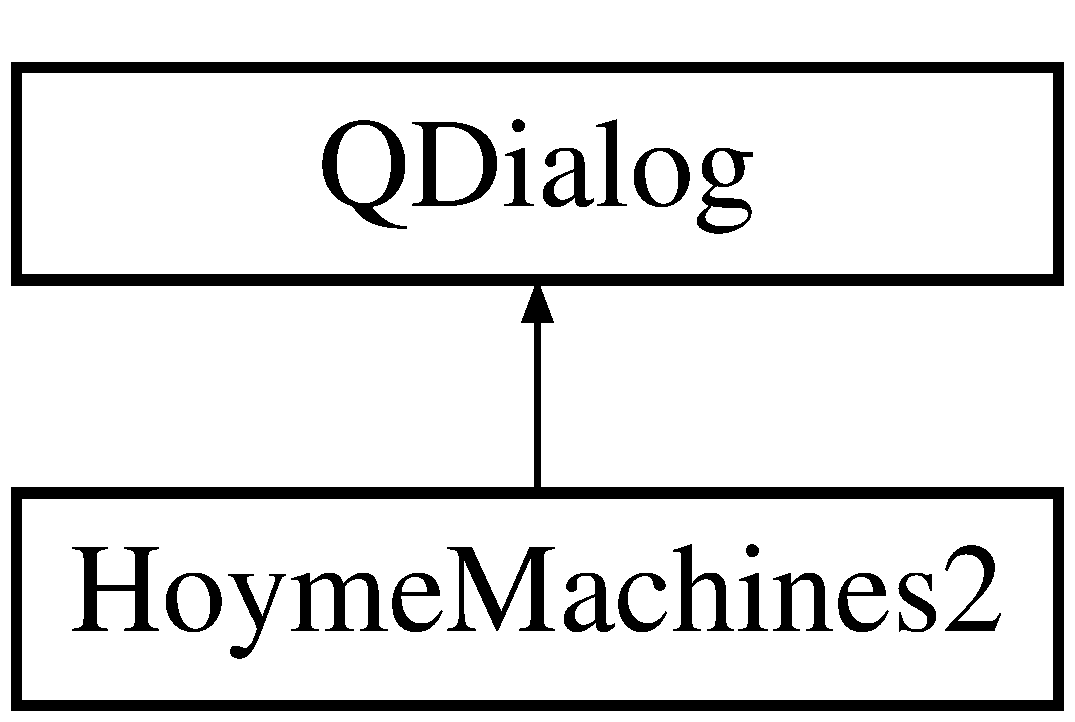
\includegraphics[height=2.000000cm]{classHoymeMachines2}
\end{center}
\end{figure}
\subsection*{Public Member Functions}
\begin{DoxyCompactItemize}
\item 
\hyperlink{classHoymeMachines2_a32862a1bf56faae9c5f2e19b35c9aa79}{Hoyme\+Machines2} (Q\+Widget $\ast$parent=0)
\item 
\hyperlink{classHoymeMachines2_a2bf57e034cd78d797fdf2927b3c0c196}{$\sim$\+Hoyme\+Machines2} ()
\end{DoxyCompactItemize}
\subsection*{Private Slots}
\begin{DoxyCompactItemize}
\item 
void \hyperlink{classHoymeMachines2_a55756f369dc90523143981d695992d74}{on\+\_\+push\+Button\+\_\+clicked} ()
\item 
void \hyperlink{classHoymeMachines2_a37269b3dacf0da0cf74e63e656cc0913}{on\+\_\+push\+Button\+\_\+2\+\_\+clicked} ()
\item 
void \hyperlink{classHoymeMachines2_af571e9f353807491b2077b8927c3d441}{on\+\_\+push\+Button\+\_\+3\+\_\+clicked} ()
\end{DoxyCompactItemize}
\subsection*{Private Attributes}
\begin{DoxyCompactItemize}
\item 
Ui\+::\+Hoyme\+Machines2 $\ast$ \hyperlink{classHoymeMachines2_a23ed6d02b1c5761599fa024214a66d11}{ui}
\end{DoxyCompactItemize}


\subsection{Constructor \& Destructor Documentation}
\hypertarget{classHoymeMachines2_a32862a1bf56faae9c5f2e19b35c9aa79}{}\index{Hoyme\+Machines2@{Hoyme\+Machines2}!Hoyme\+Machines2@{Hoyme\+Machines2}}
\index{Hoyme\+Machines2@{Hoyme\+Machines2}!Hoyme\+Machines2@{Hoyme\+Machines2}}
\subsubsection[{Hoyme\+Machines2(\+Q\+Widget $\ast$parent=0)}]{\setlength{\rightskip}{0pt plus 5cm}Hoyme\+Machines2\+::\+Hoyme\+Machines2 (
\begin{DoxyParamCaption}
\item[{Q\+Widget $\ast$}]{parent = {\ttfamily 0}}
\end{DoxyParamCaption}
)\hspace{0.3cm}{\ttfamily [explicit]}}\label{classHoymeMachines2_a32862a1bf56faae9c5f2e19b35c9aa79}

\begin{DoxyCode}
4                                               :
5     QDialog(parent),
6     \hyperlink{classHoymeMachines2_a23ed6d02b1c5761599fa024214a66d11}{ui}(\textcolor{keyword}{new} Ui::HoymeMachines2)
7 \{
8     \hyperlink{classHoymeMachines2_a23ed6d02b1c5761599fa024214a66d11}{ui}->setupUi(\textcolor{keyword}{this});
9 \}
\end{DoxyCode}
\hypertarget{classHoymeMachines2_a2bf57e034cd78d797fdf2927b3c0c196}{}\index{Hoyme\+Machines2@{Hoyme\+Machines2}!````~Hoyme\+Machines2@{$\sim$\+Hoyme\+Machines2}}
\index{````~Hoyme\+Machines2@{$\sim$\+Hoyme\+Machines2}!Hoyme\+Machines2@{Hoyme\+Machines2}}
\subsubsection[{$\sim$\+Hoyme\+Machines2()}]{\setlength{\rightskip}{0pt plus 5cm}Hoyme\+Machines2\+::$\sim$\+Hoyme\+Machines2 (
\begin{DoxyParamCaption}
{}
\end{DoxyParamCaption}
)}\label{classHoymeMachines2_a2bf57e034cd78d797fdf2927b3c0c196}

\begin{DoxyCode}
12 \{
13     \textcolor{keyword}{delete} \hyperlink{classHoymeMachines2_a23ed6d02b1c5761599fa024214a66d11}{ui};
14 \}
\end{DoxyCode}


\subsection{Member Function Documentation}
\hypertarget{classHoymeMachines2_a37269b3dacf0da0cf74e63e656cc0913}{}\index{Hoyme\+Machines2@{Hoyme\+Machines2}!on\+\_\+push\+Button\+\_\+2\+\_\+clicked@{on\+\_\+push\+Button\+\_\+2\+\_\+clicked}}
\index{on\+\_\+push\+Button\+\_\+2\+\_\+clicked@{on\+\_\+push\+Button\+\_\+2\+\_\+clicked}!Hoyme\+Machines2@{Hoyme\+Machines2}}
\subsubsection[{on\+\_\+push\+Button\+\_\+2\+\_\+clicked}]{\setlength{\rightskip}{0pt plus 5cm}void Hoyme\+Machines2\+::on\+\_\+push\+Button\+\_\+2\+\_\+clicked (
\begin{DoxyParamCaption}
{}
\end{DoxyParamCaption}
)\hspace{0.3cm}{\ttfamily [private]}, {\ttfamily [slot]}}\label{classHoymeMachines2_a37269b3dacf0da0cf74e63e656cc0913}

\begin{DoxyCode}
24 \{
25     \hyperlink{classHoymeMachines2_a23ed6d02b1c5761599fa024214a66d11}{ui}->label\_3->setText(\textcolor{stringliteral}{"Open"});
26     \hyperlink{classHoymeMachines2_a23ed6d02b1c5761599fa024214a66d11}{ui}->label\_4->setText(\textcolor{stringliteral}{"0 minutes"});
27 \}
\end{DoxyCode}
\hypertarget{classHoymeMachines2_af571e9f353807491b2077b8927c3d441}{}\index{Hoyme\+Machines2@{Hoyme\+Machines2}!on\+\_\+push\+Button\+\_\+3\+\_\+clicked@{on\+\_\+push\+Button\+\_\+3\+\_\+clicked}}
\index{on\+\_\+push\+Button\+\_\+3\+\_\+clicked@{on\+\_\+push\+Button\+\_\+3\+\_\+clicked}!Hoyme\+Machines2@{Hoyme\+Machines2}}
\subsubsection[{on\+\_\+push\+Button\+\_\+3\+\_\+clicked}]{\setlength{\rightskip}{0pt plus 5cm}void Hoyme\+Machines2\+::on\+\_\+push\+Button\+\_\+3\+\_\+clicked (
\begin{DoxyParamCaption}
{}
\end{DoxyParamCaption}
)\hspace{0.3cm}{\ttfamily [private]}, {\ttfamily [slot]}}\label{classHoymeMachines2_af571e9f353807491b2077b8927c3d441}

\begin{DoxyCode}
30 \{
31     \hyperlink{classHoymeMachines2_a23ed6d02b1c5761599fa024214a66d11}{ui}->label\_5->setText(\textcolor{stringliteral}{"In use"});
32     \hyperlink{classHoymeMachines2_a23ed6d02b1c5761599fa024214a66d11}{ui}->label\_6->setText(\textcolor{stringliteral}{"33 minutes"});
33 \}
\end{DoxyCode}
\hypertarget{classHoymeMachines2_a55756f369dc90523143981d695992d74}{}\index{Hoyme\+Machines2@{Hoyme\+Machines2}!on\+\_\+push\+Button\+\_\+clicked@{on\+\_\+push\+Button\+\_\+clicked}}
\index{on\+\_\+push\+Button\+\_\+clicked@{on\+\_\+push\+Button\+\_\+clicked}!Hoyme\+Machines2@{Hoyme\+Machines2}}
\subsubsection[{on\+\_\+push\+Button\+\_\+clicked}]{\setlength{\rightskip}{0pt plus 5cm}void Hoyme\+Machines2\+::on\+\_\+push\+Button\+\_\+clicked (
\begin{DoxyParamCaption}
{}
\end{DoxyParamCaption}
)\hspace{0.3cm}{\ttfamily [private]}, {\ttfamily [slot]}}\label{classHoymeMachines2_a55756f369dc90523143981d695992d74}

\begin{DoxyCode}
18 \{
19     \hyperlink{classHoymeMachines2_a23ed6d02b1c5761599fa024214a66d11}{ui}->washer\_1\_status->setText(\textcolor{stringliteral}{"In use"});
20     \hyperlink{classHoymeMachines2_a23ed6d02b1c5761599fa024214a66d11}{ui}->washer\_1\_timer->setText(\textcolor{stringliteral}{"19 minutes"});
21 \}
\end{DoxyCode}


\subsection{Member Data Documentation}
\hypertarget{classHoymeMachines2_a23ed6d02b1c5761599fa024214a66d11}{}\index{Hoyme\+Machines2@{Hoyme\+Machines2}!ui@{ui}}
\index{ui@{ui}!Hoyme\+Machines2@{Hoyme\+Machines2}}
\subsubsection[{ui}]{\setlength{\rightskip}{0pt plus 5cm}Ui\+::\+Hoyme\+Machines2$\ast$ Hoyme\+Machines2\+::ui\hspace{0.3cm}{\ttfamily [private]}}\label{classHoymeMachines2_a23ed6d02b1c5761599fa024214a66d11}


The documentation for this class was generated from the following files\+:\begin{DoxyCompactItemize}
\item 
\hyperlink{hoymemachines2_8h}{hoymemachines2.\+h}\item 
\hyperlink{hoymemachines2_8cpp}{hoymemachines2.\+cpp}\end{DoxyCompactItemize}

\hypertarget{classKittFloors}{}\section{Kitt\+Floors Class Reference}
\label{classKittFloors}\index{Kitt\+Floors@{Kitt\+Floors}}


{\ttfamily \#include $<$kittfloors.\+h$>$}

Inheritance diagram for Kitt\+Floors\+:\begin{figure}[H]
\begin{center}
\leavevmode
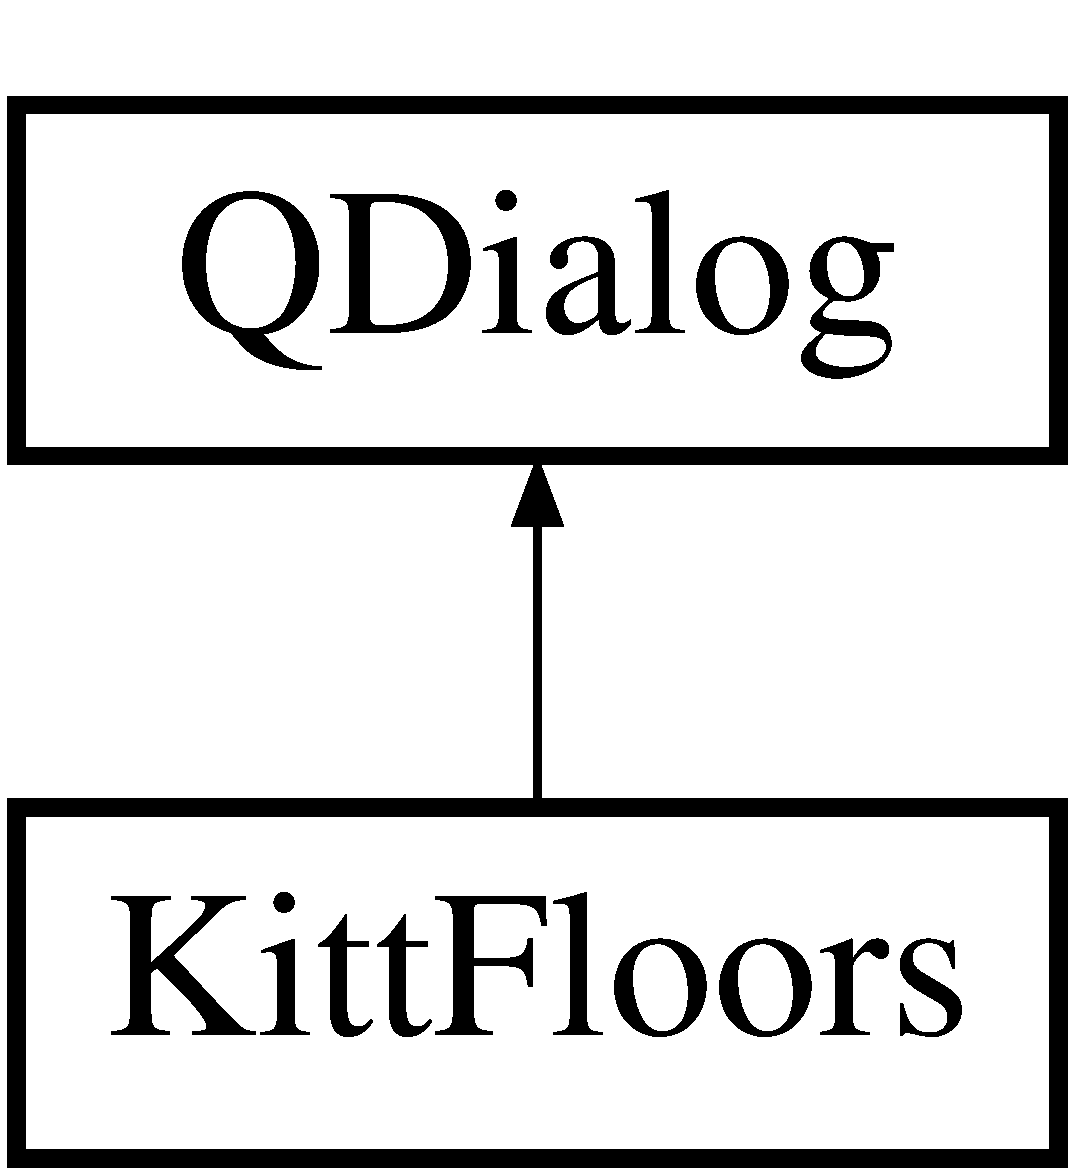
\includegraphics[height=2.000000cm]{classKittFloors}
\end{center}
\end{figure}
\subsection*{Public Member Functions}
\begin{DoxyCompactItemize}
\item 
\hyperlink{classKittFloors_aed971ec7eca6d7e02de4b442b70e1ee2}{Kitt\+Floors} (Q\+Widget $\ast$parent=0)
\item 
\hyperlink{classKittFloors_a3f6d1dd5576ce90082feee1fcdfc4b4f}{$\sim$\+Kitt\+Floors} ()
\end{DoxyCompactItemize}
\subsection*{Private Attributes}
\begin{DoxyCompactItemize}
\item 
Ui\+::\+Kitt\+Floors $\ast$ \hyperlink{classKittFloors_ac9aab8f0e6fac2b815e282d5c5913d51}{ui}
\end{DoxyCompactItemize}


\subsection{Constructor \& Destructor Documentation}
\hypertarget{classKittFloors_aed971ec7eca6d7e02de4b442b70e1ee2}{}\index{Kitt\+Floors@{Kitt\+Floors}!Kitt\+Floors@{Kitt\+Floors}}
\index{Kitt\+Floors@{Kitt\+Floors}!Kitt\+Floors@{Kitt\+Floors}}
\subsubsection[{Kitt\+Floors(\+Q\+Widget $\ast$parent=0)}]{\setlength{\rightskip}{0pt plus 5cm}Kitt\+Floors\+::\+Kitt\+Floors (
\begin{DoxyParamCaption}
\item[{Q\+Widget $\ast$}]{parent = {\ttfamily 0}}
\end{DoxyParamCaption}
)\hspace{0.3cm}{\ttfamily [explicit]}}\label{classKittFloors_aed971ec7eca6d7e02de4b442b70e1ee2}

\begin{DoxyCode}
4                                       :
5     QDialog(parent),
6     \hyperlink{classKittFloors_ac9aab8f0e6fac2b815e282d5c5913d51}{ui}(\textcolor{keyword}{new} Ui::KittFloors)
7 \{
8     \hyperlink{classKittFloors_ac9aab8f0e6fac2b815e282d5c5913d51}{ui}->setupUi(\textcolor{keyword}{this});
9 \}
\end{DoxyCode}
\hypertarget{classKittFloors_a3f6d1dd5576ce90082feee1fcdfc4b4f}{}\index{Kitt\+Floors@{Kitt\+Floors}!````~Kitt\+Floors@{$\sim$\+Kitt\+Floors}}
\index{````~Kitt\+Floors@{$\sim$\+Kitt\+Floors}!Kitt\+Floors@{Kitt\+Floors}}
\subsubsection[{$\sim$\+Kitt\+Floors()}]{\setlength{\rightskip}{0pt plus 5cm}Kitt\+Floors\+::$\sim$\+Kitt\+Floors (
\begin{DoxyParamCaption}
{}
\end{DoxyParamCaption}
)}\label{classKittFloors_a3f6d1dd5576ce90082feee1fcdfc4b4f}

\begin{DoxyCode}
12 \{
13     \textcolor{keyword}{delete} \hyperlink{classKittFloors_ac9aab8f0e6fac2b815e282d5c5913d51}{ui};
14 \}
\end{DoxyCode}


\subsection{Member Data Documentation}
\hypertarget{classKittFloors_ac9aab8f0e6fac2b815e282d5c5913d51}{}\index{Kitt\+Floors@{Kitt\+Floors}!ui@{ui}}
\index{ui@{ui}!Kitt\+Floors@{Kitt\+Floors}}
\subsubsection[{ui}]{\setlength{\rightskip}{0pt plus 5cm}Ui\+::\+Kitt\+Floors$\ast$ Kitt\+Floors\+::ui\hspace{0.3cm}{\ttfamily [private]}}\label{classKittFloors_ac9aab8f0e6fac2b815e282d5c5913d51}


The documentation for this class was generated from the following files\+:\begin{DoxyCompactItemize}
\item 
\hyperlink{kittfloors_8h}{kittfloors.\+h}\item 
\hyperlink{kittfloors_8cpp}{kittfloors.\+cpp}\end{DoxyCompactItemize}

\hypertarget{classMainWindow}{}\section{Main\+Window Class Reference}
\label{classMainWindow}\index{Main\+Window@{Main\+Window}}


{\ttfamily \#include $<$mainwindow.\+h$>$}

Inheritance diagram for Main\+Window\+:\begin{figure}[H]
\begin{center}
\leavevmode
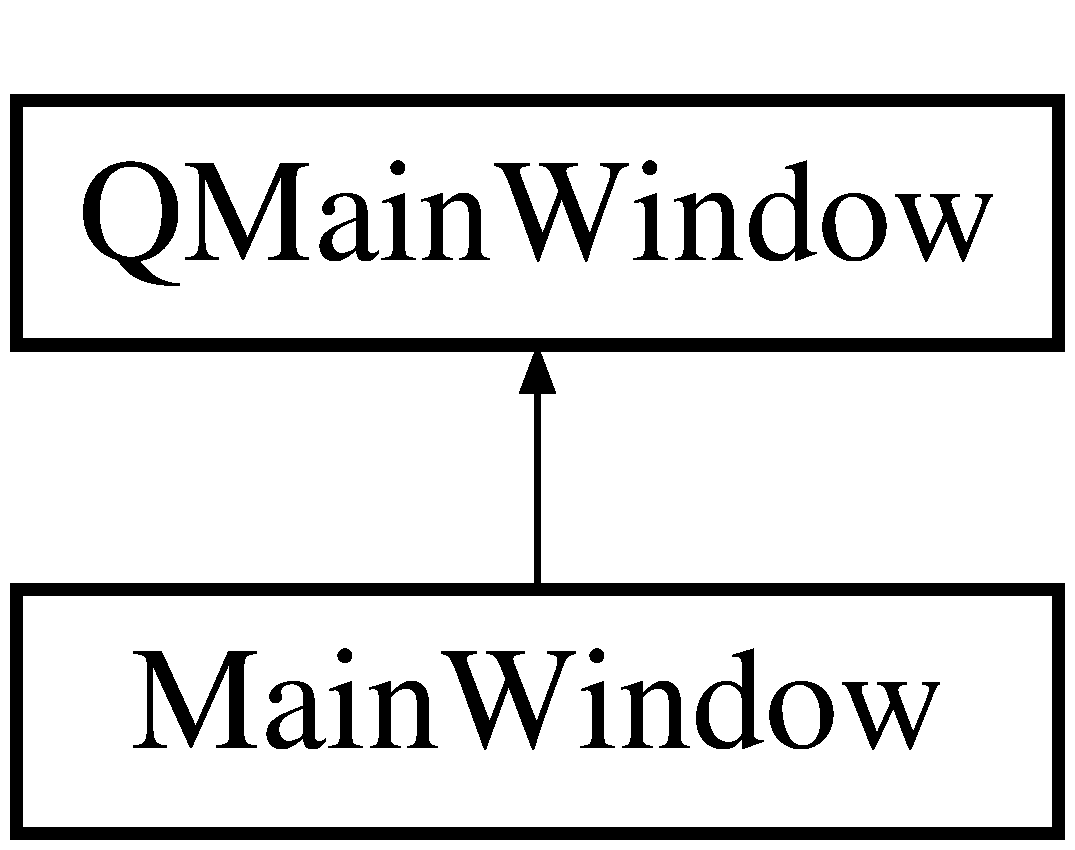
\includegraphics[height=2.000000cm]{classMainWindow}
\end{center}
\end{figure}
\subsection*{Public Member Functions}
\begin{DoxyCompactItemize}
\item 
\hyperlink{classMainWindow_a8b244be8b7b7db1b08de2a2acb9409db}{Main\+Window} (Q\+Widget $\ast$parent=0)
\item 
\hyperlink{classMainWindow_ae98d00a93bc118200eeef9f9bba1dba7}{$\sim$\+Main\+Window} ()
\end{DoxyCompactItemize}
\subsection*{Private Slots}
\begin{DoxyCompactItemize}
\item 
void \hyperlink{classMainWindow_ae907ba21cd47c6903e2744fd24cfeb78}{on\+\_\+push\+Button\+\_\+9\+\_\+clicked} ()
\item 
void \hyperlink{classMainWindow_a4de79c63c7fa0b8d7c468ac71f20be81}{on\+\_\+push\+Button\+\_\+clicked} ()
\item 
void \hyperlink{classMainWindow_ae0e46dc3da4ee07bf66e73e20300220c}{on\+\_\+push\+Button\+\_\+2\+\_\+clicked} ()
\end{DoxyCompactItemize}
\subsection*{Private Attributes}
\begin{DoxyCompactItemize}
\item 
Ui\+::\+Main\+Window $\ast$ \hyperlink{classMainWindow_a35466a70ed47252a0191168126a352a5}{ui}
\end{DoxyCompactItemize}


\subsection{Constructor \& Destructor Documentation}
\hypertarget{classMainWindow_a8b244be8b7b7db1b08de2a2acb9409db}{}\index{Main\+Window@{Main\+Window}!Main\+Window@{Main\+Window}}
\index{Main\+Window@{Main\+Window}!Main\+Window@{Main\+Window}}
\subsubsection[{Main\+Window(\+Q\+Widget $\ast$parent=0)}]{\setlength{\rightskip}{0pt plus 5cm}Main\+Window\+::\+Main\+Window (
\begin{DoxyParamCaption}
\item[{Q\+Widget $\ast$}]{parent = {\ttfamily 0}}
\end{DoxyParamCaption}
)\hspace{0.3cm}{\ttfamily [explicit]}}\label{classMainWindow_a8b244be8b7b7db1b08de2a2acb9409db}

\begin{DoxyCode}
11                                       :
12     QMainWindow(parent),
13     \hyperlink{classMainWindow_a35466a70ed47252a0191168126a352a5}{ui}(\textcolor{keyword}{new} Ui::MainWindow)
14 \{
15     \hyperlink{classMainWindow_a35466a70ed47252a0191168126a352a5}{ui}->setupUi(\textcolor{keyword}{this});
16 \}
\end{DoxyCode}
\hypertarget{classMainWindow_ae98d00a93bc118200eeef9f9bba1dba7}{}\index{Main\+Window@{Main\+Window}!````~Main\+Window@{$\sim$\+Main\+Window}}
\index{````~Main\+Window@{$\sim$\+Main\+Window}!Main\+Window@{Main\+Window}}
\subsubsection[{$\sim$\+Main\+Window()}]{\setlength{\rightskip}{0pt plus 5cm}Main\+Window\+::$\sim$\+Main\+Window (
\begin{DoxyParamCaption}
{}
\end{DoxyParamCaption}
)}\label{classMainWindow_ae98d00a93bc118200eeef9f9bba1dba7}

\begin{DoxyCode}
19 \{
20     \textcolor{keyword}{delete} \hyperlink{classMainWindow_a35466a70ed47252a0191168126a352a5}{ui};
21 \}
\end{DoxyCode}


\subsection{Member Function Documentation}
\hypertarget{classMainWindow_ae0e46dc3da4ee07bf66e73e20300220c}{}\index{Main\+Window@{Main\+Window}!on\+\_\+push\+Button\+\_\+2\+\_\+clicked@{on\+\_\+push\+Button\+\_\+2\+\_\+clicked}}
\index{on\+\_\+push\+Button\+\_\+2\+\_\+clicked@{on\+\_\+push\+Button\+\_\+2\+\_\+clicked}!Main\+Window@{Main\+Window}}
\subsubsection[{on\+\_\+push\+Button\+\_\+2\+\_\+clicked}]{\setlength{\rightskip}{0pt plus 5cm}void Main\+Window\+::on\+\_\+push\+Button\+\_\+2\+\_\+clicked (
\begin{DoxyParamCaption}
{}
\end{DoxyParamCaption}
)\hspace{0.3cm}{\ttfamily [private]}, {\ttfamily [slot]}}\label{classMainWindow_ae0e46dc3da4ee07bf66e73e20300220c}

\begin{DoxyCode}
37 \{
38     QString link = \textcolor{stringliteral}{"http://www.cs.stolaf.edu/wiki/images/2/2e/LaundryWebServiceUseM.pdf"};
39     QDesktopServices::openUrl(QUrl(link));
40 \}
\end{DoxyCode}
\hypertarget{classMainWindow_ae907ba21cd47c6903e2744fd24cfeb78}{}\index{Main\+Window@{Main\+Window}!on\+\_\+push\+Button\+\_\+9\+\_\+clicked@{on\+\_\+push\+Button\+\_\+9\+\_\+clicked}}
\index{on\+\_\+push\+Button\+\_\+9\+\_\+clicked@{on\+\_\+push\+Button\+\_\+9\+\_\+clicked}!Main\+Window@{Main\+Window}}
\subsubsection[{on\+\_\+push\+Button\+\_\+9\+\_\+clicked}]{\setlength{\rightskip}{0pt plus 5cm}void Main\+Window\+::on\+\_\+push\+Button\+\_\+9\+\_\+clicked (
\begin{DoxyParamCaption}
{}
\end{DoxyParamCaption}
)\hspace{0.3cm}{\ttfamily [private]}, {\ttfamily [slot]}}\label{classMainWindow_ae907ba21cd47c6903e2744fd24cfeb78}

\begin{DoxyCode}
24 \{
25     \hyperlink{classHoymeFloors}{HoymeFloors} hFl;
26     hFl.setModal(\textcolor{keyword}{true});
27     hFl.exec();
28 \}
\end{DoxyCode}
\hypertarget{classMainWindow_a4de79c63c7fa0b8d7c468ac71f20be81}{}\index{Main\+Window@{Main\+Window}!on\+\_\+push\+Button\+\_\+clicked@{on\+\_\+push\+Button\+\_\+clicked}}
\index{on\+\_\+push\+Button\+\_\+clicked@{on\+\_\+push\+Button\+\_\+clicked}!Main\+Window@{Main\+Window}}
\subsubsection[{on\+\_\+push\+Button\+\_\+clicked}]{\setlength{\rightskip}{0pt plus 5cm}void Main\+Window\+::on\+\_\+push\+Button\+\_\+clicked (
\begin{DoxyParamCaption}
{}
\end{DoxyParamCaption}
)\hspace{0.3cm}{\ttfamily [private]}, {\ttfamily [slot]}}\label{classMainWindow_a4de79c63c7fa0b8d7c468ac71f20be81}

\begin{DoxyCode}
31 \{
32     QString link = \textcolor{stringliteral}{"http://www.cs.stolaf.edu/wiki/index.php/LaundryB"};
33     QDesktopServices::openUrl(QUrl(link));
34 \}
\end{DoxyCode}


\subsection{Member Data Documentation}
\hypertarget{classMainWindow_a35466a70ed47252a0191168126a352a5}{}\index{Main\+Window@{Main\+Window}!ui@{ui}}
\index{ui@{ui}!Main\+Window@{Main\+Window}}
\subsubsection[{ui}]{\setlength{\rightskip}{0pt plus 5cm}Ui\+::\+Main\+Window$\ast$ Main\+Window\+::ui\hspace{0.3cm}{\ttfamily [private]}}\label{classMainWindow_a35466a70ed47252a0191168126a352a5}


The documentation for this class was generated from the following files\+:\begin{DoxyCompactItemize}
\item 
\hyperlink{mainwindow_8h}{mainwindow.\+h}\item 
\hyperlink{mainwindow_8cpp}{mainwindow.\+cpp}\end{DoxyCompactItemize}

\hypertarget{classServerSocket}{}\section{Server\+Socket Class Reference}
\label{classServerSocket}\index{Server\+Socket@{Server\+Socket}}


{\ttfamily \#include $<$Socket.\+h$>$}

Inheritance diagram for Server\+Socket\+:\begin{figure}[H]
\begin{center}
\leavevmode
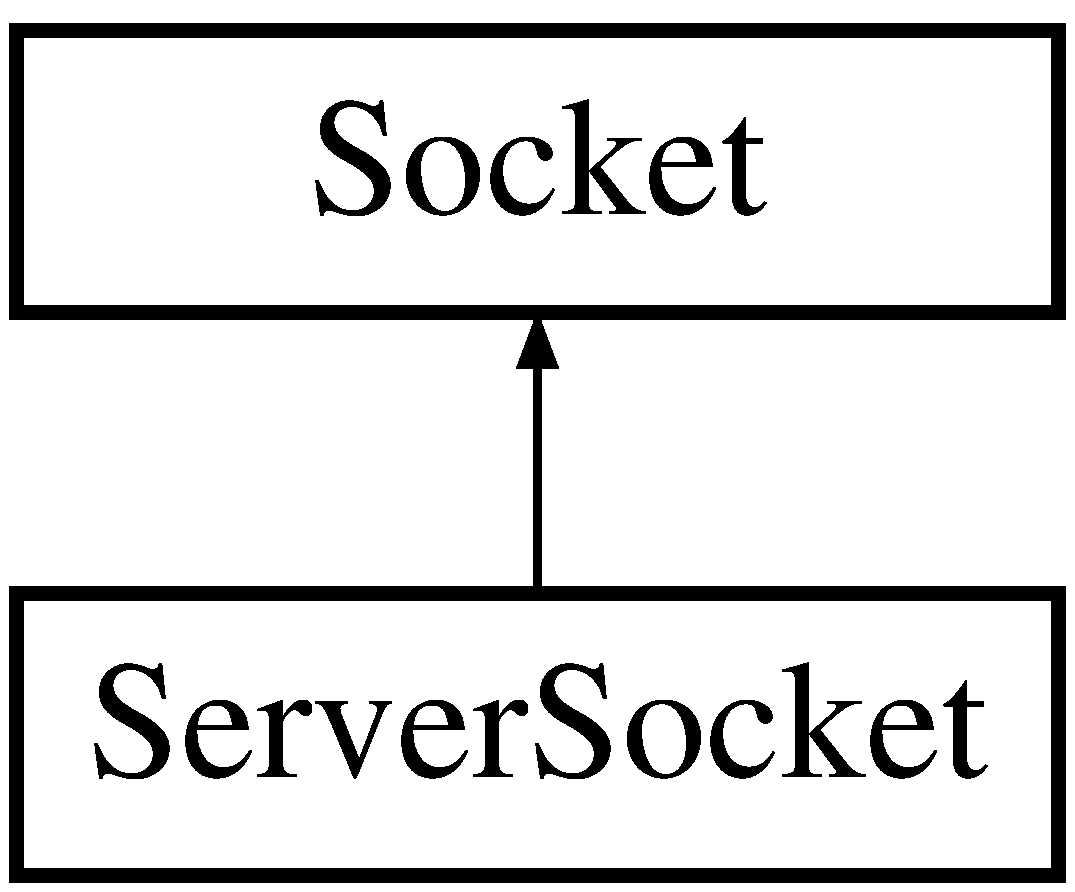
\includegraphics[height=2.000000cm]{classServerSocket}
\end{center}
\end{figure}
\subsection*{Public Member Functions}
\begin{DoxyCompactItemize}
\item 
\hyperlink{classServerSocket_a2b3098589541243241ca25495155186c}{Server\+Socket} ()
\item 
\hyperlink{classServerSocket_a3dc1a31f740e4a8d69ae10c5dcb547d6}{Server\+Socket} (int port)
\item 
int \hyperlink{classServerSocket_a6cd7ad5bd162805cb4fa9f126205e046}{bind} (int port)
\item 
\hyperlink{classSocket}{Socket} $\ast$ \hyperlink{classServerSocket_accc3d56d42aa50a5f3c920cf0b26959b}{accept} ()
\item 
int \hyperlink{classServerSocket_a3eac38fb0cc7686f758f1bc77e1b1f6b}{get\+Bound} ()
\end{DoxyCompactItemize}
\subsection*{Protected Attributes}
\begin{DoxyCompactItemize}
\item 
int \hyperlink{classServerSocket_ae7e043fe5c2a7abdcc3d83219fe5106f}{bound}
\end{DoxyCompactItemize}
\subsection*{Additional Inherited Members}


\subsection{Constructor \& Destructor Documentation}
\hypertarget{classServerSocket_a2b3098589541243241ca25495155186c}{}\index{Server\+Socket@{Server\+Socket}!Server\+Socket@{Server\+Socket}}
\index{Server\+Socket@{Server\+Socket}!Server\+Socket@{Server\+Socket}}
\subsubsection[{Server\+Socket()}]{\setlength{\rightskip}{0pt plus 5cm}Server\+Socket\+::\+Server\+Socket (
\begin{DoxyParamCaption}
{}
\end{DoxyParamCaption}
)\hspace{0.3cm}{\ttfamily [inline]}}\label{classServerSocket_a2b3098589541243241ca25495155186c}

\begin{DoxyCode}
62 : \hyperlink{classSocket_a93c96fe7bea2fc834c88786629fa041e}{Socket}() \{ \hyperlink{classServerSocket_ae7e043fe5c2a7abdcc3d83219fe5106f}{bound} = 0; \}
\end{DoxyCode}
\hypertarget{classServerSocket_a3dc1a31f740e4a8d69ae10c5dcb547d6}{}\index{Server\+Socket@{Server\+Socket}!Server\+Socket@{Server\+Socket}}
\index{Server\+Socket@{Server\+Socket}!Server\+Socket@{Server\+Socket}}
\subsubsection[{Server\+Socket(int port)}]{\setlength{\rightskip}{0pt plus 5cm}Server\+Socket\+::\+Server\+Socket (
\begin{DoxyParamCaption}
\item[{int}]{port}
\end{DoxyParamCaption}
)}\label{classServerSocket_a3dc1a31f740e4a8d69ae10c5dcb547d6}
initialize a socket and attempt to associate a port with it 
\begin{DoxyParams}{Parameters}
{\em port} & T\+C\+P port number \\
\hline
\end{DoxyParams}

\begin{DoxyCode}
112                                    : \hyperlink{classSocket_a93c96fe7bea2fc834c88786629fa041e}{Socket}() \{
113   \hyperlink{classServerSocket_ae7e043fe5c2a7abdcc3d83219fe5106f}{bound} = 0;
114   \hyperlink{classServerSocket_a6cd7ad5bd162805cb4fa9f126205e046}{bind}(port);
115 \}
\end{DoxyCode}


\subsection{Member Function Documentation}
\hypertarget{classServerSocket_accc3d56d42aa50a5f3c920cf0b26959b}{}\index{Server\+Socket@{Server\+Socket}!accept@{accept}}
\index{accept@{accept}!Server\+Socket@{Server\+Socket}}
\subsubsection[{accept()}]{\setlength{\rightskip}{0pt plus 5cm}{\bf Socket} $\ast$ Server\+Socket\+::accept (
\begin{DoxyParamCaption}
{}
\end{DoxyParamCaption}
)}\label{classServerSocket_accc3d56d42aa50a5f3c920cf0b26959b}
Wait for and accept one connection request from another process, potentially on a different host \begin{DoxyReturn}{Returns}
Address of a newly allocated \hyperlink{classSocket}{Socket} for communication with another process. Return 0 if attempt to accept failed or if this server socket is not bound 
\end{DoxyReturn}

\begin{DoxyCode}
141                              \{
142   \textcolor{keywordflow}{if} (!\hyperlink{classServerSocket_ae7e043fe5c2a7abdcc3d83219fe5106f}{bound})
143     \textcolor{keywordflow}{return} 0;
144 
145   \textcolor{keyword}{struct }sockaddr\_in ca; \textcolor{comment}{// socket address structure for the new client}
146   socklen\_t size = \textcolor{keyword}{sizeof}(\textcolor{keyword}{struct }sockaddr);
147   \textcolor{keywordtype}{int} clientd;
148 
149   cout << \textcolor{stringliteral}{"Waiting for a incoming connection..."} << endl;
150   \textcolor{keywordflow}{if} ((clientd = ::\hyperlink{classServerSocket_accc3d56d42aa50a5f3c920cf0b26959b}{accept}(\hyperlink{classSocket_a457f5e3f2429eb859f9e80f064073874}{descrip}, (\textcolor{keyword}{struct} sockaddr *)&ca, &size)) < 0) \{
151     cerr << \textcolor{stringliteral}{"ServerSocket::accept() "} << strerror(errno) << endl;
152     \textcolor{keywordflow}{return} 0;
153   \}
154   \textcolor{comment}{// ::accept() attempt was successful}
155   \textcolor{comment}{/* Note:  Could retrieve the IP address of client from ca, size */}
156 
157   \textcolor{keywordflow}{return} \textcolor{keyword}{new} \hyperlink{classSocket_a93c96fe7bea2fc834c88786629fa041e}{Socket}(clientd);
158 \}
\end{DoxyCode}
\hypertarget{classServerSocket_a6cd7ad5bd162805cb4fa9f126205e046}{}\index{Server\+Socket@{Server\+Socket}!bind@{bind}}
\index{bind@{bind}!Server\+Socket@{Server\+Socket}}
\subsubsection[{bind(int port)}]{\setlength{\rightskip}{0pt plus 5cm}int Server\+Socket\+::bind (
\begin{DoxyParamCaption}
\item[{int}]{port}
\end{DoxyParamCaption}
)}\label{classServerSocket_a6cd7ad5bd162805cb4fa9f126205e046}
Associate a port with this server socket \begin{DoxyPrecond}{Precondition}
State variable connected must be assigned before calling this method 
\end{DoxyPrecond}

\begin{DoxyParams}{Parameters}
{\em port} & T\+C\+P port number \\
\hline
\end{DoxyParams}
\begin{DoxyReturn}{Returns}
1 on success, 0 on failure 
\end{DoxyReturn}

\begin{DoxyCode}
117                                \{
118   \textcolor{keywordflow}{if} (\hyperlink{classServerSocket_ae7e043fe5c2a7abdcc3d83219fe5106f}{bound}) \{
119     cerr << \textcolor{stringliteral}{"ServerSocket::bind() - already marked as bound, skipping"} << endl;
120     \textcolor{keywordflow}{return} 0;
121   \}
122   \textcolor{comment}{// bound == 0}
123 
124   \textcolor{keyword}{struct }sockaddr\_in sa;
125   sa.sin\_family = AF\_INET;
126   sa.sin\_port = htons(port);
127   sa.sin\_addr.s\_addr = INADDR\_ANY;
128 
129   \textcolor{keywordflow}{if} (::\hyperlink{classServerSocket_a6cd7ad5bd162805cb4fa9f126205e046}{bind}(\hyperlink{classSocket_a457f5e3f2429eb859f9e80f064073874}{descrip}, (\textcolor{keyword}{struct} sockaddr *)&sa, \textcolor{keyword}{sizeof}(sa)) < 0) \{
130     cerr << \textcolor{stringliteral}{"ServerSocket::bind() bind "} << strerror(errno) << endl;
131     \textcolor{keywordflow}{return} 0;
132   \}
133   \textcolor{keywordflow}{if} (::listen(\hyperlink{classSocket_a457f5e3f2429eb859f9e80f064073874}{descrip}, 5) < 0) \{
134     cerr << \textcolor{stringliteral}{"ServerSocket::bind() listen "} << strerror(errno) << endl;
135     \textcolor{keywordflow}{return} 0;
136   \}
137   \hyperlink{classServerSocket_ae7e043fe5c2a7abdcc3d83219fe5106f}{bound} = 1;
138   \textcolor{keywordflow}{return} 1;
139 \}
\end{DoxyCode}
\hypertarget{classServerSocket_a3eac38fb0cc7686f758f1bc77e1b1f6b}{}\index{Server\+Socket@{Server\+Socket}!get\+Bound@{get\+Bound}}
\index{get\+Bound@{get\+Bound}!Server\+Socket@{Server\+Socket}}
\subsubsection[{get\+Bound()}]{\setlength{\rightskip}{0pt plus 5cm}int Server\+Socket\+::get\+Bound (
\begin{DoxyParamCaption}
{}
\end{DoxyParamCaption}
)\hspace{0.3cm}{\ttfamily [inline]}}\label{classServerSocket_a3eac38fb0cc7686f758f1bc77e1b1f6b}
\begin{DoxyReturn}{Returns}
Value of state variable bound 
\end{DoxyReturn}

\begin{DoxyCode}
81 \{ \textcolor{keywordflow}{return} \hyperlink{classServerSocket_ae7e043fe5c2a7abdcc3d83219fe5106f}{bound}; \}
\end{DoxyCode}


\subsection{Member Data Documentation}
\hypertarget{classServerSocket_ae7e043fe5c2a7abdcc3d83219fe5106f}{}\index{Server\+Socket@{Server\+Socket}!bound@{bound}}
\index{bound@{bound}!Server\+Socket@{Server\+Socket}}
\subsubsection[{bound}]{\setlength{\rightskip}{0pt plus 5cm}int Server\+Socket\+::bound\hspace{0.3cm}{\ttfamily [protected]}}\label{classServerSocket_ae7e043fe5c2a7abdcc3d83219fe5106f}
non-\/zero if \hyperlink{classServerSocket_a6cd7ad5bd162805cb4fa9f126205e046}{bind()} succeeded on this socket 

The documentation for this class was generated from the following files\+:\begin{DoxyCompactItemize}
\item 
\hyperlink{Socket_8h}{Socket.\+h}\item 
\hyperlink{Socket_8cpp}{Socket.\+cpp}\end{DoxyCompactItemize}

\hypertarget{classSocket}{}\section{Socket Class Reference}
\label{classSocket}\index{Socket@{Socket}}


{\ttfamily \#include $<$Socket.\+h$>$}

Inheritance diagram for Socket\+:\begin{figure}[H]
\begin{center}
\leavevmode
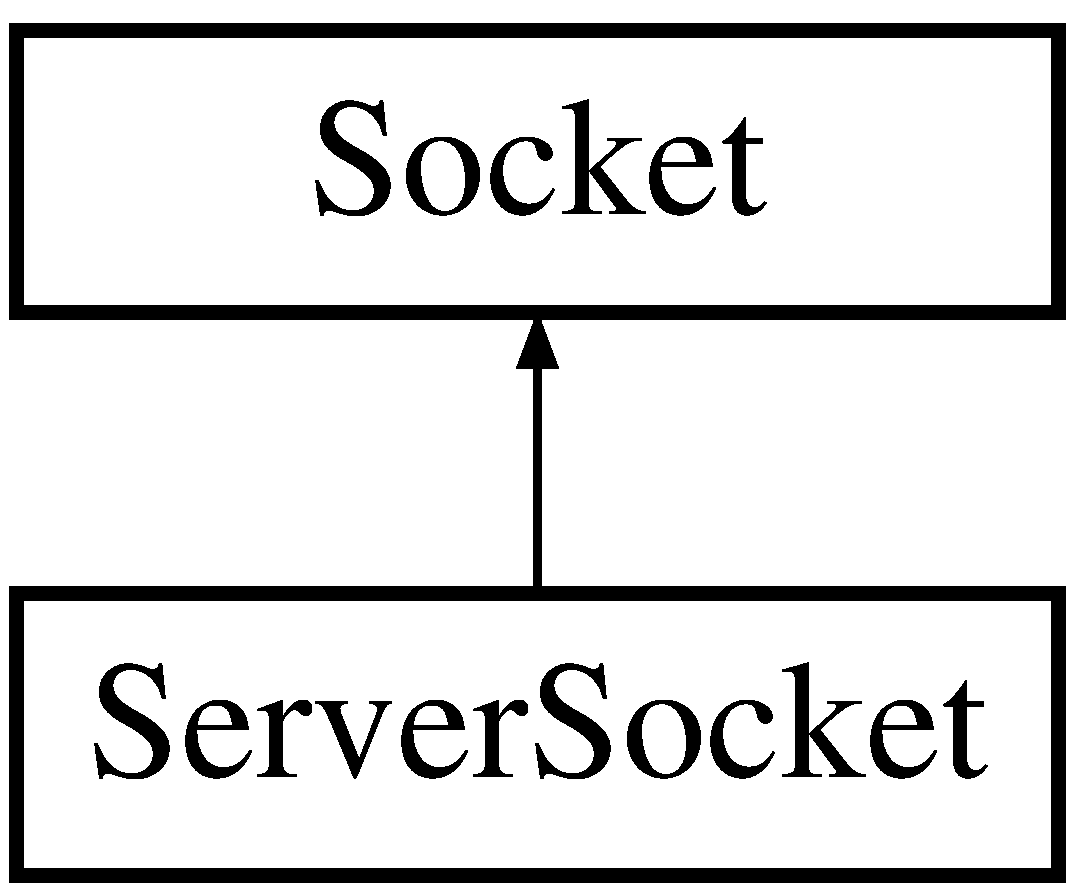
\includegraphics[height=2.000000cm]{classSocket}
\end{center}
\end{figure}
\subsection*{Public Member Functions}
\begin{DoxyCompactItemize}
\item 
\hyperlink{classSocket_a93c96fe7bea2fc834c88786629fa041e}{Socket} (int sd=-\/1)
\item 
\hyperlink{classSocket_aeac4eb6379a543d38ed88977d3b6630a}{$\sim$\+Socket} ()
\item 
\hyperlink{classSocket_a9016e6a1e5ae817f917449d5e3a7a380}{Socket} (const char $\ast$host, int port)
\item 
int \hyperlink{classSocket_abc97e53080c01a06cc8f5efea7c6cdf0}{connect} (const char $\ast$host, int port)
\item 
int \hyperlink{classSocket_aca3e5b9c5459a50bd8fb03d29ef9e48e}{send} (const char $\ast$msg, int len)
\item 
int \hyperlink{classSocket_a1830972b26797cde234054f81f0921de}{recv} (char $\ast$msg, int len)
\item 
void \hyperlink{classSocket_a75ee749264ccbcfc4dfbf5442e55dcb8}{close} ()
\item 
int \hyperlink{classSocket_a378077061dfb9c50e9db4b0d84ff2b03}{get\+Descriptor} ()
\item 
int \hyperlink{classSocket_a2b89fc6d75015cbf6abe93b2b9994ef4}{get\+Connected} ()
\end{DoxyCompactItemize}
\subsection*{Protected Member Functions}
\begin{DoxyCompactItemize}
\item 
void \hyperlink{classSocket_a23f2fbf5f8449277c7d140f32d12fca3}{create\+\_\+socket} ()
\end{DoxyCompactItemize}
\subsection*{Protected Attributes}
\begin{DoxyCompactItemize}
\item 
int \hyperlink{classSocket_a457f5e3f2429eb859f9e80f064073874}{descrip}
\item 
int \hyperlink{classSocket_af04394b9f1235562146aaa9291df70f8}{connected}
\end{DoxyCompactItemize}


\subsection{Detailed Description}
A class for socket communication 

\subsection{Constructor \& Destructor Documentation}
\hypertarget{classSocket_a93c96fe7bea2fc834c88786629fa041e}{}\index{Socket@{Socket}!Socket@{Socket}}
\index{Socket@{Socket}!Socket@{Socket}}
\subsubsection[{Socket(int sd=-\/1)}]{\setlength{\rightskip}{0pt plus 5cm}Socket\+::\+Socket (
\begin{DoxyParamCaption}
\item[{int}]{sd = {\ttfamily -\/1}}
\end{DoxyParamCaption}
)}\label{classSocket_a93c96fe7bea2fc834c88786629fa041e}

\begin{DoxyCode}
23                      \{
24   \textcolor{keywordflow}{if} (sd == -1) \{
25     \hyperlink{classSocket_a23f2fbf5f8449277c7d140f32d12fca3}{create\_socket}();
26   \} \textcolor{keywordflow}{else} \{
27     \hyperlink{classSocket_a457f5e3f2429eb859f9e80f064073874}{descrip} = sd;
28     \textcolor{keyword}{struct }sockaddr\_in ca; \textcolor{comment}{// socket address structure for the new client}
29     socklen\_t size = \textcolor{keyword}{sizeof}(\textcolor{keyword}{struct }sockaddr);
30     \textcolor{keywordflow}{if} (!::getpeername(sd, (\textcolor{keyword}{struct} sockaddr *)&ca, &size)) \{
31       \hyperlink{classSocket_af04394b9f1235562146aaa9291df70f8}{connected} = 1;
32     \} \textcolor{keywordflow}{else} \{
33       \hyperlink{classSocket_af04394b9f1235562146aaa9291df70f8}{connected} = 0;
34       \textcolor{keywordflow}{if} (errno != ENOTCONN)
35         cerr << \textcolor{stringliteral}{"Socket::Socket() getpeername "} << strerror(errno) << endl;
36     \}
37   \}
38 \}
\end{DoxyCode}
\hypertarget{classSocket_aeac4eb6379a543d38ed88977d3b6630a}{}\index{Socket@{Socket}!````~Socket@{$\sim$\+Socket}}
\index{````~Socket@{$\sim$\+Socket}!Socket@{Socket}}
\subsubsection[{$\sim$\+Socket()}]{\setlength{\rightskip}{0pt plus 5cm}Socket\+::$\sim$\+Socket (
\begin{DoxyParamCaption}
{}
\end{DoxyParamCaption}
)}\label{classSocket_aeac4eb6379a543d38ed88977d3b6630a}

\begin{DoxyCode}
45                 \{
46   \hyperlink{classSocket_a75ee749264ccbcfc4dfbf5442e55dcb8}{close}();
47 \}
\end{DoxyCode}
\hypertarget{classSocket_a9016e6a1e5ae817f917449d5e3a7a380}{}\index{Socket@{Socket}!Socket@{Socket}}
\index{Socket@{Socket}!Socket@{Socket}}
\subsubsection[{Socket(const char $\ast$host, int port)}]{\setlength{\rightskip}{0pt plus 5cm}Socket\+::\+Socket (
\begin{DoxyParamCaption}
\item[{const char $\ast$}]{host, }
\item[{int}]{port}
\end{DoxyParamCaption}
)}\label{classSocket_a9016e6a1e5ae817f917449d5e3a7a380}
initialize a socket and attempt to connect to a particular host and port 
\begin{DoxyParams}{Parameters}
{\em host} & Internet name for a computer, e.\+g., rns202-\/1.\+cs.\+stolaf.\+edu \\
\hline
{\em port} & T\+C\+P port for server socket on host \\
\hline
\end{DoxyParams}

\begin{DoxyCode}
40                                          \{
41   \hyperlink{classSocket_a23f2fbf5f8449277c7d140f32d12fca3}{create\_socket}();
42   \hyperlink{classSocket_abc97e53080c01a06cc8f5efea7c6cdf0}{connect}(host, port);
43 \}
\end{DoxyCode}


\subsection{Member Function Documentation}
\hypertarget{classSocket_a75ee749264ccbcfc4dfbf5442e55dcb8}{}\index{Socket@{Socket}!close@{close}}
\index{close@{close}!Socket@{Socket}}
\subsubsection[{close()}]{\setlength{\rightskip}{0pt plus 5cm}void Socket\+::close (
\begin{DoxyParamCaption}
{}
\end{DoxyParamCaption}
)}\label{classSocket_a75ee749264ccbcfc4dfbf5442e55dcb8}
Invalidate this socket for further use. If connected, first shut down communication. 
\begin{DoxyCode}
49                    \{
50   \textcolor{keywordflow}{if} (\hyperlink{classSocket_af04394b9f1235562146aaa9291df70f8}{connected} and ::shutdown(\hyperlink{classSocket_a457f5e3f2429eb859f9e80f064073874}{descrip}, SHUT\_RDWR) < 0)
51     cerr << \textcolor{stringliteral}{"Socket::close() shutdown "} << strerror(errno) << endl;
52   \hyperlink{classSocket_af04394b9f1235562146aaa9291df70f8}{connected} = 0;
53   \textcolor{keywordflow}{if} (::\hyperlink{classSocket_a75ee749264ccbcfc4dfbf5442e55dcb8}{close}(\hyperlink{classSocket_a457f5e3f2429eb859f9e80f064073874}{descrip}) < 0)
54     cerr << \textcolor{stringliteral}{"Socket::close() "} << strerror(errno) << endl;
55   \textcolor{comment}{// cout << "closed socket <" << descrip << ">" << endl; // DEBUG}
56 \}
\end{DoxyCode}
\hypertarget{classSocket_abc97e53080c01a06cc8f5efea7c6cdf0}{}\index{Socket@{Socket}!connect@{connect}}
\index{connect@{connect}!Socket@{Socket}}
\subsubsection[{connect(const char $\ast$host, int port)}]{\setlength{\rightskip}{0pt plus 5cm}int Socket\+::connect (
\begin{DoxyParamCaption}
\item[{const char $\ast$}]{host, }
\item[{int}]{port}
\end{DoxyParamCaption}
)}\label{classSocket_abc97e53080c01a06cc8f5efea7c6cdf0}
Connect this socket to a server \begin{DoxyPrecond}{Precondition}
State variable connected must be assigned before calling this method 
\end{DoxyPrecond}

\begin{DoxyParams}{Parameters}
{\em host} & Internet name for a computer, e.\+g., rns202-\/1.\+cs.\+stolaf.\+edu \\
\hline
{\em port} & T\+C\+P port for server socket on host \\
\hline
\end{DoxyParams}
\begin{DoxyReturn}{Returns}
1 on success, 0 on failure 
\end{DoxyReturn}

\begin{DoxyCode}
58                                               \{
59   \textcolor{keywordflow}{if} (\hyperlink{classSocket_af04394b9f1235562146aaa9291df70f8}{connected}) \{
60     cerr << \textcolor{stringliteral}{"Socket::connect() - already marked as connected, skipping"} << endl;
61     \textcolor{keywordflow}{return} 0;
62   \}
63   \textcolor{comment}{// connected == 0}
64 
65   \textcolor{keyword}{struct }hostent *hp;
66   \textcolor{keyword}{struct }sockaddr\_in sa;
67   \textcolor{keywordflow}{if} ((hp = gethostbyname(host)) == NULL) \{
68     cerr << \textcolor{stringliteral}{"Socket::connect() gethostbyname() "} << strerror(errno) << endl;
69     \textcolor{keywordflow}{return} 0;
70   \}
71   memset((\textcolor{keywordtype}{char} *)&sa, \textcolor{charliteral}{'\(\backslash\)0'}, \textcolor{keyword}{sizeof}(sa));
72   memcpy((\textcolor{keywordtype}{char} *)&sa.sin\_addr.s\_addr, hp->h\_addr, hp->h\_length);
73   sa.sin\_family = AF\_INET;
74   sa.sin\_port = htons(port);
75 
76   \textcolor{keywordflow}{if} (::\hyperlink{classSocket_abc97e53080c01a06cc8f5efea7c6cdf0}{connect}(\hyperlink{classSocket_a457f5e3f2429eb859f9e80f064073874}{descrip}, (\textcolor{keyword}{struct} sockaddr *)&sa, \textcolor{keyword}{sizeof}(sa)) < 0) \{
77     cerr << \textcolor{stringliteral}{"Socket::connect() "} << strerror(errno) << endl;
78     \textcolor{keywordflow}{if} (errno == EISCONN)
79       \hyperlink{classSocket_af04394b9f1235562146aaa9291df70f8}{connected} = 1;
80     \textcolor{keywordflow}{return} 0;
81   \}
82   \hyperlink{classSocket_af04394b9f1235562146aaa9291df70f8}{connected} = 1;
83   \textcolor{keywordflow}{return} 1;
84 \}
\end{DoxyCode}
\hypertarget{classSocket_a23f2fbf5f8449277c7d140f32d12fca3}{}\index{Socket@{Socket}!create\+\_\+socket@{create\+\_\+socket}}
\index{create\+\_\+socket@{create\+\_\+socket}!Socket@{Socket}}
\subsubsection[{create\+\_\+socket()}]{\setlength{\rightskip}{0pt plus 5cm}void Socket\+::create\+\_\+socket (
\begin{DoxyParamCaption}
{}
\end{DoxyParamCaption}
)\hspace{0.3cm}{\ttfamily [protected]}}\label{classSocket_a23f2fbf5f8449277c7d140f32d12fca3}
helper method for socket initialization \begin{DoxyParagraph}{State Changes}
Initialize descrip, and assign 0 to connected 
\end{DoxyParagraph}

\begin{DoxyCode}
17                            \{
18   \textcolor{keywordflow}{if} ((\hyperlink{classSocket_a457f5e3f2429eb859f9e80f064073874}{descrip} = socket(AF\_INET, SOCK\_STREAM, 0)) < 0)
19     cerr << \textcolor{stringliteral}{"Socket::Socket():"} << strerror(errno) << endl;
20   \hyperlink{classSocket_af04394b9f1235562146aaa9291df70f8}{connected} = 0;
21 \}
\end{DoxyCode}
\hypertarget{classSocket_a2b89fc6d75015cbf6abe93b2b9994ef4}{}\index{Socket@{Socket}!get\+Connected@{get\+Connected}}
\index{get\+Connected@{get\+Connected}!Socket@{Socket}}
\subsubsection[{get\+Connected()}]{\setlength{\rightskip}{0pt plus 5cm}int Socket\+::get\+Connected (
\begin{DoxyParamCaption}
{}
\end{DoxyParamCaption}
)\hspace{0.3cm}{\ttfamily [inline]}}\label{classSocket_a2b89fc6d75015cbf6abe93b2b9994ef4}
\begin{DoxyReturn}{Returns}
Value of state variable connected 
\end{DoxyReturn}

\begin{DoxyCode}
49 \{ \textcolor{keywordflow}{return} \hyperlink{classSocket_af04394b9f1235562146aaa9291df70f8}{connected}; \}
\end{DoxyCode}
\hypertarget{classSocket_a378077061dfb9c50e9db4b0d84ff2b03}{}\index{Socket@{Socket}!get\+Descriptor@{get\+Descriptor}}
\index{get\+Descriptor@{get\+Descriptor}!Socket@{Socket}}
\subsubsection[{get\+Descriptor()}]{\setlength{\rightskip}{0pt plus 5cm}int Socket\+::get\+Descriptor (
\begin{DoxyParamCaption}
{}
\end{DoxyParamCaption}
)\hspace{0.3cm}{\ttfamily [inline]}}\label{classSocket_a378077061dfb9c50e9db4b0d84ff2b03}
\begin{DoxyReturn}{Returns}
Value of state variable descrip 
\end{DoxyReturn}

\begin{DoxyCode}
46 \{ \textcolor{keywordflow}{return} \hyperlink{classSocket_a457f5e3f2429eb859f9e80f064073874}{descrip}; \}
\end{DoxyCode}
\hypertarget{classSocket_a1830972b26797cde234054f81f0921de}{}\index{Socket@{Socket}!recv@{recv}}
\index{recv@{recv}!Socket@{Socket}}
\subsubsection[{recv(char $\ast$msg, int len)}]{\setlength{\rightskip}{0pt plus 5cm}int Socket\+::recv (
\begin{DoxyParamCaption}
\item[{char $\ast$}]{msg, }
\item[{int}]{len}
\end{DoxyParamCaption}
)}\label{classSocket_a1830972b26797cde234054f81f0921de}
Receive a message on this socket 
\begin{DoxyParams}{Parameters}
{\em buff} & Array to receive message \\
\hline
{\em len} & Maximum number of characters to receive in buff \\
\hline
\end{DoxyParams}
\begin{DoxyReturn}{Returns}
Number of characters transmitted, or -\/1 on failure 
\end{DoxyReturn}

\begin{DoxyCode}
98                                     \{
99   \textcolor{keywordflow}{if} (!\hyperlink{classSocket_af04394b9f1235562146aaa9291df70f8}{connected}) \{
100     cerr << \textcolor{stringliteral}{"Attempt to recv() on a disconnected Socket"} << endl;
101     \textcolor{keywordflow}{return} -1;
102   \}
103 
104   \textcolor{keywordtype}{int} ret;
105   \textcolor{keywordflow}{if} ((ret = ::\hyperlink{classSocket_a1830972b26797cde234054f81f0921de}{recv}(\hyperlink{classSocket_a457f5e3f2429eb859f9e80f064073874}{descrip}, buff, len, 0)) < 0) \{
106     cerr << \textcolor{stringliteral}{"Socket::recv() "} << strerror(errno) << endl;
107     \textcolor{keywordflow}{return} -1;
108   \}
109   \textcolor{keywordflow}{return} ret;
110 \}
\end{DoxyCode}
\hypertarget{classSocket_aca3e5b9c5459a50bd8fb03d29ef9e48e}{}\index{Socket@{Socket}!send@{send}}
\index{send@{send}!Socket@{Socket}}
\subsubsection[{send(const char $\ast$msg, int len)}]{\setlength{\rightskip}{0pt plus 5cm}int Socket\+::send (
\begin{DoxyParamCaption}
\item[{const char $\ast$}]{msg, }
\item[{int}]{len}
\end{DoxyParamCaption}
)}\label{classSocket_aca3e5b9c5459a50bd8fb03d29ef9e48e}
Send a message on this socket 
\begin{DoxyParams}{Parameters}
{\em msg} & Message to be transmitted \\
\hline
{\em len} & Number of characters of msg to transmit \\
\hline
\end{DoxyParams}
\begin{DoxyReturn}{Returns}
Number of characters transmitted, or -\/1 on failure 
\end{DoxyReturn}

\begin{DoxyCode}
86                                          \{
87   \textcolor{keywordflow}{if} (!\hyperlink{classSocket_af04394b9f1235562146aaa9291df70f8}{connected}) \{
88     cerr << \textcolor{stringliteral}{"Attempt to send() on a disconnected Socket"} << endl;
89     \textcolor{keywordflow}{return} -1;
90   \}
91 
92   \textcolor{keywordtype}{int} ret;
93   \textcolor{keywordflow}{if} ((ret = ::\hyperlink{classSocket_aca3e5b9c5459a50bd8fb03d29ef9e48e}{send}(\hyperlink{classSocket_a457f5e3f2429eb859f9e80f064073874}{descrip}, msg, len, 0)) < 0)
94     cerr << \textcolor{stringliteral}{"Socket::send() "} << strerror(errno) << endl;
95   \textcolor{keywordflow}{return} ret;
96 \}
\end{DoxyCode}


\subsection{Member Data Documentation}
\hypertarget{classSocket_af04394b9f1235562146aaa9291df70f8}{}\index{Socket@{Socket}!connected@{connected}}
\index{connected@{connected}!Socket@{Socket}}
\subsubsection[{connected}]{\setlength{\rightskip}{0pt plus 5cm}int Socket\+::connected\hspace{0.3cm}{\ttfamily [protected]}}\label{classSocket_af04394b9f1235562146aaa9291df70f8}
non-\/zero if \hyperlink{classSocket_abc97e53080c01a06cc8f5efea7c6cdf0}{connect()} succeeded on this socket \hypertarget{classSocket_a457f5e3f2429eb859f9e80f064073874}{}\index{Socket@{Socket}!descrip@{descrip}}
\index{descrip@{descrip}!Socket@{Socket}}
\subsubsection[{descrip}]{\setlength{\rightskip}{0pt plus 5cm}int Socket\+::descrip\hspace{0.3cm}{\ttfamily [protected]}}\label{classSocket_a457f5e3f2429eb859f9e80f064073874}
socket descriptor, or -\/1 if failed to allocate socket 

The documentation for this class was generated from the following files\+:\begin{DoxyCompactItemize}
\item 
\hyperlink{Socket_8h}{Socket.\+h}\item 
\hyperlink{Socket_8cpp}{Socket.\+cpp}\end{DoxyCompactItemize}

\hypertarget{classWorker}{}\section{Worker Class Reference}
\label{classWorker}\index{Worker@{Worker}}


{\ttfamily \#include $<$Worker.\+h$>$}

Inheritance diagram for Worker\+:\begin{figure}[H]
\begin{center}
\leavevmode
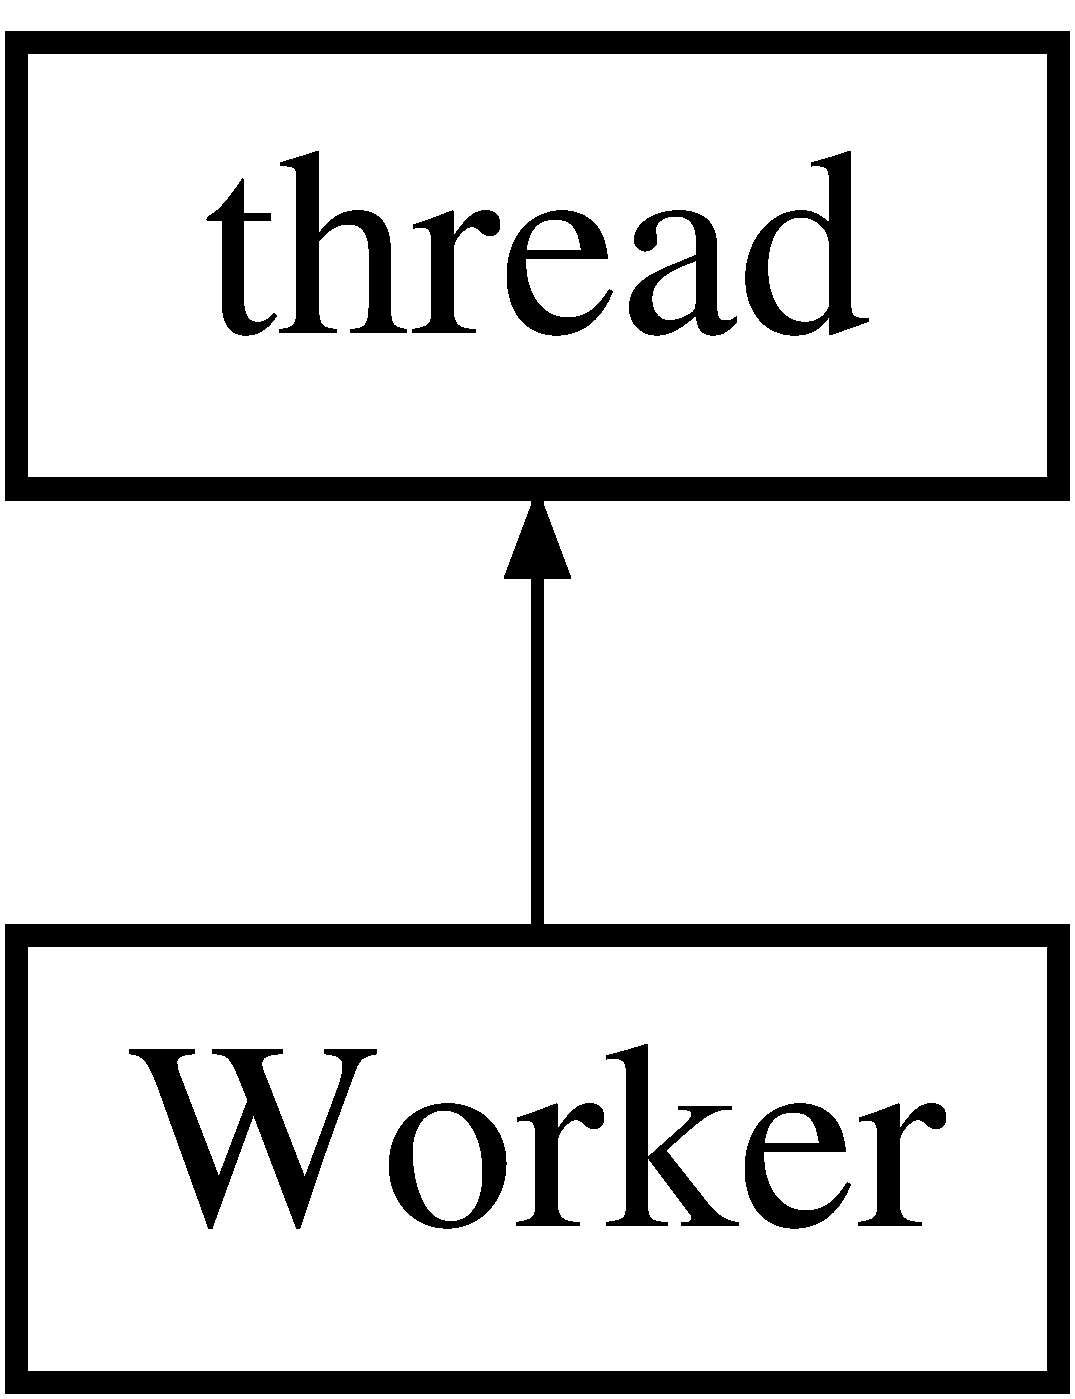
\includegraphics[height=2.000000cm]{classWorker}
\end{center}
\end{figure}
\subsection*{Public Member Functions}
\begin{DoxyCompactItemize}
\item 
\hyperlink{classWorker_a0a75e3ee66254224da70636e3ce40d8e}{Worker} (int i=-\/1, \hyperlink{classSocket}{Socket} $\ast$sp=0, const \hyperlink{structControlData}{Control\+Data} $\ast$cdp=0)
\item 
\hyperlink{classWorker_aa8e4543ef1e93fd9d884269ba30c5bfe}{$\sim$\+Worker} ()
\item 
\hyperlink{Worker_8h_ab3804a8a4369184ad46dadf8e54957b6}{Thread\+State} \hyperlink{classWorker_a2ababbc935eb10458640d2441f5e0c95}{get\+State} ()
\item 
int \hyperlink{classWorker_ac4629e67476bbb1daab8ed28545b8421}{get\+Id} ()
\end{DoxyCompactItemize}
\subsection*{Protected Member Functions}
\begin{DoxyCompactItemize}
\item 
void \hyperlink{classWorker_aeeb8e21ecb6687c34db1ad301028e41b}{do\+Work} (const \hyperlink{structControlData}{Control\+Data} $\ast$cdp)
\end{DoxyCompactItemize}
\subsection*{Protected Attributes}
\begin{DoxyCompactItemize}
\item 
int \hyperlink{classWorker_a50acebd9c077214060ff190bd54d351c}{id}
\item 
\hyperlink{classSocket}{Socket} $\ast$ \hyperlink{classWorker_a4562eb405aea20c7ac8a552e2075898f}{sockp}
\item 
\hyperlink{Worker_8h_ab3804a8a4369184ad46dadf8e54957b6}{Thread\+State} \hyperlink{classWorker_aeb90d4cd08a8a4759749c5388be8c78d}{state}
\end{DoxyCompactItemize}
\subsection*{Static Protected Attributes}
\begin{DoxyCompactItemize}
\item 
static int \hyperlink{classWorker_a2749db22d3591fe663b9a25e90a88e9d}{M\+A\+X\+B\+U\+F\+F} = 100
\end{DoxyCompactItemize}


\subsection{Detailed Description}
A class representing a thread that implements services for a client 

\subsection{Constructor \& Destructor Documentation}
\hypertarget{classWorker_a0a75e3ee66254224da70636e3ce40d8e}{}\index{Worker@{Worker}!Worker@{Worker}}
\index{Worker@{Worker}!Worker@{Worker}}
\subsubsection[{Worker(int i=-\/1, Socket $\ast$sp=0, const Control\+Data $\ast$cdp=0)}]{\setlength{\rightskip}{0pt plus 5cm}Worker\+::\+Worker (
\begin{DoxyParamCaption}
\item[{int}]{i = {\ttfamily -\/1}, }
\item[{{\bf Socket} $\ast$}]{sp = {\ttfamily 0}, }
\item[{const {\bf Control\+Data} $\ast$}]{cdp = {\ttfamily 0}}
\end{DoxyParamCaption}
)}\label{classWorker_a0a75e3ee66254224da70636e3ce40d8e}

\begin{DoxyParams}{Parameters}
{\em i} & I\+D number for this worker thread \\
\hline
{\em sp} & Pointer to socket for communicating with client \\
\hline
\end{DoxyParams}

\begin{DoxyCode}
11 : thread(&\hyperlink{classWorker_aeeb8e21ecb6687c34db1ad301028e41b}{Worker::doWork}, \textcolor{keyword}{this}, cdp), \hyperlink{classWorker_a50acebd9c077214060ff190bd54d351c}{id}(i), \hyperlink{classWorker_a4562eb405aea20c7ac8a552e2075898f}{sockp}(sp), 
      \hyperlink{classWorker_aeb90d4cd08a8a4759749c5388be8c78d}{state}(\hyperlink{Worker_8h_ab3804a8a4369184ad46dadf8e54957b6a1061be6c3fb88d32829cba6f6b2be304}{RUNNING}) \{\}
\end{DoxyCode}
\hypertarget{classWorker_aa8e4543ef1e93fd9d884269ba30c5bfe}{}\index{Worker@{Worker}!````~Worker@{$\sim$\+Worker}}
\index{````~Worker@{$\sim$\+Worker}!Worker@{Worker}}
\subsubsection[{$\sim$\+Worker()}]{\setlength{\rightskip}{0pt plus 5cm}Worker\+::$\sim$\+Worker (
\begin{DoxyParamCaption}
{}
\end{DoxyParamCaption}
)}\label{classWorker_aa8e4543ef1e93fd9d884269ba30c5bfe}

\begin{DoxyCode}
18                    \{
19     \textcolor{keyword}{delete} \hyperlink{classWorker_a4562eb405aea20c7ac8a552e2075898f}{sockp};
20     \hyperlink{classWorker_a4562eb405aea20c7ac8a552e2075898f}{sockp} = 0;
21   \}
\end{DoxyCode}


\subsection{Member Function Documentation}
\hypertarget{classWorker_aeeb8e21ecb6687c34db1ad301028e41b}{}\index{Worker@{Worker}!do\+Work@{do\+Work}}
\index{do\+Work@{do\+Work}!Worker@{Worker}}
\subsubsection[{do\+Work(const Control\+Data $\ast$cdp)}]{\setlength{\rightskip}{0pt plus 5cm}void Worker\+::do\+Work (
\begin{DoxyParamCaption}
\item[{const {\bf Control\+Data} $\ast$}]{cdp}
\end{DoxyParamCaption}
)\hspace{0.3cm}{\ttfamily [protected]}}\label{classWorker_aeeb8e21ecb6687c34db1ad301028e41b}

\begin{DoxyParams}{Parameters}
{\em cdp} & Points to shared data structure for controlling server \\
\hline
\end{DoxyParams}

\begin{DoxyCode}
23                                             \{
24   \textcolor{keywordtype}{char} buff[\hyperlink{classWorker_a2749db22d3591fe663b9a25e90a88e9d}{MAXBUFF}];  \textcolor{comment}{/* message buffer */}
25   \textcolor{keywordtype}{int} ret;  \textcolor{comment}{/* return value from a call */}
26 
27     cout << \textcolor{stringliteral}{"["} << \textcolor{keywordtype}{id} << \textcolor{stringliteral}{"] started"} << endl;
28   \textcolor{comment}{// cout << "[" << id << "] socket <" << sockp->getDescriptor() << ">" << endl; //DEBUG}
29 
30 
31   \textcolor{comment}{// send welcome message}
32     \textcolor{keywordflow}{if} (cdp->\hyperlink{structControlData_ac8fbf80345423cf5650ae64bfb10dc88}{contin}) 
33       strcpy(buff, \textcolor{stringliteral}{"ACK"});
34     \textcolor{keywordflow}{else}
35       strcpy(buff, \textcolor{stringliteral}{"DONE"});
36     \hyperlink{classWorker_a4562eb405aea20c7ac8a552e2075898f}{sockp}->\hyperlink{classSocket_aca3e5b9c5459a50bd8fb03d29ef9e48e}{send}(buff, strlen(buff));  
37 
38     \textcolor{keywordflow}{while} (strcmp(buff, \textcolor{stringliteral}{"DONE"}) != 0) \{
39       ret = \hyperlink{classWorker_a4562eb405aea20c7ac8a552e2075898f}{sockp}->\hyperlink{classSocket_a1830972b26797cde234054f81f0921de}{recv}(buff, \hyperlink{classWorker_a2749db22d3591fe663b9a25e90a88e9d}{MAXBUFF}-1);
40 
41     buff[ret] = \textcolor{charliteral}{'\(\backslash\)0'};  \textcolor{comment}{// add terminating nullbyte to received array of chars}
42     cout << \textcolor{stringliteral}{"["} << \textcolor{keywordtype}{id} << \textcolor{stringliteral}{"] Received message ("} << ret << \textcolor{stringliteral}{" chars):"} << endl 
43     << buff << endl;
44 
45     \textcolor{keywordflow}{if} (strcmp(buff, \textcolor{stringliteral}{"DONE"}) == 0 || !cdp->\hyperlink{structControlData_ac8fbf80345423cf5650ae64bfb10dc88}{contin}) \{
46       strcpy(buff, \textcolor{stringliteral}{"DONE"});
47       \hyperlink{classWorker_a4562eb405aea20c7ac8a552e2075898f}{sockp}->\hyperlink{classSocket_aca3e5b9c5459a50bd8fb03d29ef9e48e}{send}(buff, 4);
48       cout << \textcolor{stringliteral}{"["} << \textcolor{keywordtype}{id} << \textcolor{stringliteral}{"] sent termination message"} << endl;
49     \} \textcolor{keywordflow}{else} \textcolor{keywordflow}{if} (strncmp(buff, \textcolor{stringliteral}{"MSG "}, 4) == 0) \{
50       \hyperlink{classWorker_a4562eb405aea20c7ac8a552e2075898f}{sockp}->\hyperlink{classSocket_aca3e5b9c5459a50bd8fb03d29ef9e48e}{send}(\textcolor{stringliteral}{"ACK"}, 3);
51       cout << \textcolor{stringliteral}{"["} << \textcolor{keywordtype}{id} << \textcolor{stringliteral}{"] sent acknowledgment"} << endl;
52     \} \textcolor{keywordflow}{else} \textcolor{keywordflow}{if} (strncmp(buff, \textcolor{stringliteral}{"LINE1 "}, 6) == 0) \{
53 
54       ifstream f;
55       \textcolor{keywordtype}{char} fileName[20];
56       \textcolor{keywordflow}{for} (\textcolor{keywordtype}{int} n=6; buff[n] != \textcolor{charliteral}{'\(\backslash\)0'}; ++n)\{
57         fileName[n-6] = buff[n];
58       \}
59       f.open(fileName);
60       \textcolor{keywordflow}{if} (f.is\_open()) \{
61         \textcolor{keywordtype}{string} line;
62         getline(f, line);
63         cout << line << endl;
64         \textcolor{keywordtype}{int} n = line.length();
65         \hyperlink{classWorker_a4562eb405aea20c7ac8a552e2075898f}{sockp}->\hyperlink{classSocket_aca3e5b9c5459a50bd8fb03d29ef9e48e}{send}(line.c\_str(), n);
66         cout<<\textcolor{stringliteral}{"["}<<\textcolor{keywordtype}{id}<<\textcolor{stringliteral}{"] Returned line from file "}<<fileName<<endl;
67         f.close();
68       \}
69       \textcolor{keywordflow}{else} \{
70         \hyperlink{classWorker_a4562eb405aea20c7ac8a552e2075898f}{sockp}->\hyperlink{classSocket_aca3e5b9c5459a50bd8fb03d29ef9e48e}{send}(\textcolor{stringliteral}{"NACK"}, 4);
71         cout<<\textcolor{stringliteral}{"Worker: send negative NACK"}<<endl;
72       \}
73     \} \textcolor{keywordflow}{else} \{
74       \hyperlink{classWorker_a4562eb405aea20c7ac8a552e2075898f}{sockp}->\hyperlink{classSocket_aca3e5b9c5459a50bd8fb03d29ef9e48e}{send}(\textcolor{stringliteral}{"NACK"}, 4);
75       cout << \textcolor{stringliteral}{"["} << \textcolor{keywordtype}{id} << \textcolor{stringliteral}{"] sent negative acknowledgment"} << endl;
76     \}
77 
78   \}
79 
80   \textcolor{comment}{// receive END message from client}
81   \textcolor{keywordflow}{if} ((ret = \hyperlink{classWorker_a4562eb405aea20c7ac8a552e2075898f}{sockp}->\hyperlink{classSocket_a1830972b26797cde234054f81f0921de}{recv}(buff, \hyperlink{classWorker_a2749db22d3591fe663b9a25e90a88e9d}{MAXBUFF}-1)) != -1) \{
82     buff[ret] = \textcolor{charliteral}{'\(\backslash\)0'};
83     cout << \textcolor{stringliteral}{"["} << \textcolor{keywordtype}{id} << \textcolor{stringliteral}{"] Received "} << buff << \textcolor{stringliteral}{" from client"} << endl;
84   \}
85   \hyperlink{classWorker_aeb90d4cd08a8a4759749c5388be8c78d}{state} = \hyperlink{Worker_8h_ab3804a8a4369184ad46dadf8e54957b6a9c954bcf443428c80b0f107b3bc48749}{DONE};
86 \}
\end{DoxyCode}
\hypertarget{classWorker_ac4629e67476bbb1daab8ed28545b8421}{}\index{Worker@{Worker}!get\+Id@{get\+Id}}
\index{get\+Id@{get\+Id}!Worker@{Worker}}
\subsubsection[{get\+Id()}]{\setlength{\rightskip}{0pt plus 5cm}int Worker\+::get\+Id (
\begin{DoxyParamCaption}
{}
\end{DoxyParamCaption}
)\hspace{0.3cm}{\ttfamily [inline]}}\label{classWorker_ac4629e67476bbb1daab8ed28545b8421}

\begin{DoxyCode}
40 \{ \textcolor{keywordflow}{return} \hyperlink{classWorker_a50acebd9c077214060ff190bd54d351c}{id}; \}
\end{DoxyCode}
\hypertarget{classWorker_a2ababbc935eb10458640d2441f5e0c95}{}\index{Worker@{Worker}!get\+State@{get\+State}}
\index{get\+State@{get\+State}!Worker@{Worker}}
\subsubsection[{get\+State()}]{\setlength{\rightskip}{0pt plus 5cm}{\bf Thread\+State} Worker\+::get\+State (
\begin{DoxyParamCaption}
{}
\end{DoxyParamCaption}
)\hspace{0.3cm}{\ttfamily [inline]}}\label{classWorker_a2ababbc935eb10458640d2441f5e0c95}

\begin{DoxyCode}
39 \{ \textcolor{keywordflow}{return} \hyperlink{classWorker_aeb90d4cd08a8a4759749c5388be8c78d}{state}; \}
\end{DoxyCode}


\subsection{Member Data Documentation}
\hypertarget{classWorker_a50acebd9c077214060ff190bd54d351c}{}\index{Worker@{Worker}!id@{id}}
\index{id@{id}!Worker@{Worker}}
\subsubsection[{id}]{\setlength{\rightskip}{0pt plus 5cm}int Worker\+::id\hspace{0.3cm}{\ttfamily [protected]}}\label{classWorker_a50acebd9c077214060ff190bd54d351c}
unique identifier for this worker thread \hypertarget{classWorker_a2749db22d3591fe663b9a25e90a88e9d}{}\index{Worker@{Worker}!M\+A\+X\+B\+U\+F\+F@{M\+A\+X\+B\+U\+F\+F}}
\index{M\+A\+X\+B\+U\+F\+F@{M\+A\+X\+B\+U\+F\+F}!Worker@{Worker}}
\subsubsection[{M\+A\+X\+B\+U\+F\+F}]{\setlength{\rightskip}{0pt plus 5cm}int Worker\+::\+M\+A\+X\+B\+U\+F\+F = 100\hspace{0.3cm}{\ttfamily [static]}, {\ttfamily [protected]}}\label{classWorker_a2749db22d3591fe663b9a25e90a88e9d}
buffer size for socket communication \hypertarget{classWorker_a4562eb405aea20c7ac8a552e2075898f}{}\index{Worker@{Worker}!sockp@{sockp}}
\index{sockp@{sockp}!Worker@{Worker}}
\subsubsection[{sockp}]{\setlength{\rightskip}{0pt plus 5cm}{\bf Socket}$\ast$ Worker\+::sockp\hspace{0.3cm}{\ttfamily [protected]}}\label{classWorker_a4562eb405aea20c7ac8a552e2075898f}
socket for communicating with client \hypertarget{classWorker_aeb90d4cd08a8a4759749c5388be8c78d}{}\index{Worker@{Worker}!state@{state}}
\index{state@{state}!Worker@{Worker}}
\subsubsection[{state}]{\setlength{\rightskip}{0pt plus 5cm}{\bf Thread\+State} Worker\+::state\hspace{0.3cm}{\ttfamily [protected]}}\label{classWorker_aeb90d4cd08a8a4759749c5388be8c78d}
current status of this worker thread 

The documentation for this class was generated from the following files\+:\begin{DoxyCompactItemize}
\item 
\hyperlink{Worker_8h}{Worker.\+h}\item 
\hyperlink{Worker_8cpp}{Worker.\+cpp}\end{DoxyCompactItemize}

\chapter{File Documentation}
\hypertarget{CLIENT_8cpp}{}\section{C\+L\+I\+E\+N\+T.\+cpp File Reference}
\label{CLIENT_8cpp}\index{C\+L\+I\+E\+N\+T.\+cpp@{C\+L\+I\+E\+N\+T.\+cpp}}
{\ttfamily \#include \char`\"{}C\+L\+I\+E\+N\+T.\+h\char`\"{}}\\*
{\ttfamily \#include $<$sstream$>$}\\*

\hypertarget{CLIENT_8h}{}\section{C\+L\+I\+E\+N\+T.\+h File Reference}
\label{CLIENT_8h}\index{C\+L\+I\+E\+N\+T.\+h@{C\+L\+I\+E\+N\+T.\+h}}
{\ttfamily \#include $<$iostream$>$}\\*
{\ttfamily \#include $<$cstring$>$}\\*
{\ttfamily \#include $<$vector$>$}\\*
{\ttfamily \#include $<$string$>$}\\*
{\ttfamily \#include $<$sstream$>$}\\*
{\ttfamily \#include \char`\"{}Socket.\+h\char`\"{}}\\*
\subsection*{Classes}
\begin{DoxyCompactItemize}
\item 
class \hyperlink{classCLIENT}{C\+L\+I\+E\+N\+T}
\end{DoxyCompactItemize}

\hypertarget{CLIENT1_8cpp}{}\section{C\+L\+I\+E\+N\+T1.\+cpp File Reference}
\label{CLIENT1_8cpp}\index{C\+L\+I\+E\+N\+T1.\+cpp@{C\+L\+I\+E\+N\+T1.\+cpp}}
{\ttfamily \#include \char`\"{}C\+L\+I\+E\+N\+T.\+h\char`\"{}}\\*
{\ttfamily \#include $<$sstream$>$}\\*

\hypertarget{CLIENT2_8cpp}{}\section{C\+L\+I\+E\+N\+T2.\+cpp File Reference}
\label{CLIENT2_8cpp}\index{C\+L\+I\+E\+N\+T2.\+cpp@{C\+L\+I\+E\+N\+T2.\+cpp}}
{\ttfamily \#include \char`\"{}C\+L\+I\+E\+N\+T.\+h\char`\"{}}\\*
{\ttfamily \#include $<$sstream$>$}\\*

\hypertarget{CLIENTDriver_8cpp}{}\section{C\+L\+I\+E\+N\+T\+Driver.\+cpp File Reference}
\label{CLIENTDriver_8cpp}\index{C\+L\+I\+E\+N\+T\+Driver.\+cpp@{C\+L\+I\+E\+N\+T\+Driver.\+cpp}}
{\ttfamily \#include \char`\"{}C\+L\+I\+E\+N\+T.\+h\char`\"{}}\\*
\subsection*{Functions}
\begin{DoxyCompactItemize}
\item 
int \hyperlink{CLIENTDriver_8cpp_ae66f6b31b5ad750f1fe042a706a4e3d4}{main} ()
\end{DoxyCompactItemize}


\subsection{Function Documentation}
\hypertarget{CLIENTDriver_8cpp_ae66f6b31b5ad750f1fe042a706a4e3d4}{}\index{C\+L\+I\+E\+N\+T\+Driver.\+cpp@{C\+L\+I\+E\+N\+T\+Driver.\+cpp}!main@{main}}
\index{main@{main}!C\+L\+I\+E\+N\+T\+Driver.\+cpp@{C\+L\+I\+E\+N\+T\+Driver.\+cpp}}
\subsubsection[{main()}]{\setlength{\rightskip}{0pt plus 5cm}int main (
\begin{DoxyParamCaption}
{}
\end{DoxyParamCaption}
)}\label{CLIENTDriver_8cpp_ae66f6b31b5ad750f1fe042a706a4e3d4}

\begin{DoxyCode}
3           \{
4     \hyperlink{classCLIENT}{CLIENT} client1 (\textcolor{stringliteral}{"rns203-13.cs.stolaf.edu"}, 25276, \textcolor{stringliteral}{"LINE1 ell-02-123-l.txt"} ); 
5     cout << client1.returnMachineStatus() << endl; 
6     cout << client1.returnMachineTimer() << endl; 
7 \}
\end{DoxyCode}

\hypertarget{hoymefloors_8cpp}{}\section{hoymefloors.\+cpp File Reference}
\label{hoymefloors_8cpp}\index{hoymefloors.\+cpp@{hoymefloors.\+cpp}}
{\ttfamily \#include \char`\"{}hoymefloors.\+h\char`\"{}}\\*
{\ttfamily \#include \char`\"{}ui\+\_\+hoymefloors.\+h\char`\"{}}\\*
{\ttfamily \#include \char`\"{}hoymemachines.\+h\char`\"{}}\\*
{\ttfamily \#include \char`\"{}hoymemachines2.\+h\char`\"{}}\\*

\hypertarget{hoymefloors_8h}{}\section{hoymefloors.\+h File Reference}
\label{hoymefloors_8h}\index{hoymefloors.\+h@{hoymefloors.\+h}}
{\ttfamily \#include $<$Q\+Dialog$>$}\\*
\subsection*{Classes}
\begin{DoxyCompactItemize}
\item 
class \hyperlink{classHoymeFloors}{Hoyme\+Floors}
\end{DoxyCompactItemize}
\subsection*{Namespaces}
\begin{DoxyCompactItemize}
\item 
 \hyperlink{namespaceUi}{Ui}
\end{DoxyCompactItemize}

\hypertarget{hoymemachines_8cpp}{}\section{hoymemachines.\+cpp File Reference}
\label{hoymemachines_8cpp}\index{hoymemachines.\+cpp@{hoymemachines.\+cpp}}
{\ttfamily \#include \char`\"{}hoymemachines.\+h\char`\"{}}\\*
{\ttfamily \#include \char`\"{}ui\+\_\+hoymemachines.\+h\char`\"{}}\\*
{\ttfamily \#include $<$iostream$>$}\\*
{\ttfamily \#include $<$cstring$>$}\\*
{\ttfamily \#include $<$vector$>$}\\*
{\ttfamily \#include $<$string$>$}\\*
{\ttfamily \#include $<$sstream$>$}\\*
{\ttfamily \#include $<$C\+L\+I\+E\+N\+T.\+h$>$}\\*

\hypertarget{hoymemachines_8h}{}\section{hoymemachines.\+h File Reference}
\label{hoymemachines_8h}\index{hoymemachines.\+h@{hoymemachines.\+h}}
{\ttfamily \#include $<$Q\+Dialog$>$}\\*
\subsection*{Classes}
\begin{DoxyCompactItemize}
\item 
class \hyperlink{classHoymeMachines}{Hoyme\+Machines}
\end{DoxyCompactItemize}
\subsection*{Namespaces}
\begin{DoxyCompactItemize}
\item 
 \hyperlink{namespaceUi}{Ui}
\end{DoxyCompactItemize}

\hypertarget{hoymemachines2_8cpp}{}\section{hoymemachines2.\+cpp File Reference}
\label{hoymemachines2_8cpp}\index{hoymemachines2.\+cpp@{hoymemachines2.\+cpp}}
{\ttfamily \#include \char`\"{}hoymemachines2.\+h\char`\"{}}\\*
{\ttfamily \#include \char`\"{}ui\+\_\+hoymemachines2.\+h\char`\"{}}\\*

\hypertarget{hoymemachines2_8h}{}\section{hoymemachines2.\+h File Reference}
\label{hoymemachines2_8h}\index{hoymemachines2.\+h@{hoymemachines2.\+h}}
{\ttfamily \#include $<$Q\+Dialog$>$}\\*
\subsection*{Classes}
\begin{DoxyCompactItemize}
\item 
class \hyperlink{classHoymeMachines2}{Hoyme\+Machines2}
\end{DoxyCompactItemize}
\subsection*{Namespaces}
\begin{DoxyCompactItemize}
\item 
 \hyperlink{namespaceUi}{Ui}
\end{DoxyCompactItemize}

\hypertarget{kittfloors_8cpp}{}\section{kittfloors.\+cpp File Reference}
\label{kittfloors_8cpp}\index{kittfloors.\+cpp@{kittfloors.\+cpp}}
{\ttfamily \#include \char`\"{}kittfloors.\+h\char`\"{}}\\*
{\ttfamily \#include \char`\"{}ui\+\_\+kittfloors.\+h\char`\"{}}\\*

\hypertarget{kittfloors_8h}{}\section{kittfloors.\+h File Reference}
\label{kittfloors_8h}\index{kittfloors.\+h@{kittfloors.\+h}}
{\ttfamily \#include $<$Q\+Dialog$>$}\\*
\subsection*{Classes}
\begin{DoxyCompactItemize}
\item 
class \hyperlink{classKittFloors}{Kitt\+Floors}
\end{DoxyCompactItemize}
\subsection*{Namespaces}
\begin{DoxyCompactItemize}
\item 
 \hyperlink{namespaceUi}{Ui}
\end{DoxyCompactItemize}

\hypertarget{main_8cpp}{}\section{main.\+cpp File Reference}
\label{main_8cpp}\index{main.\+cpp@{main.\+cpp}}
{\ttfamily \#include \char`\"{}mainwindow.\+h\char`\"{}}\\*
{\ttfamily \#include $<$Q\+Application$>$}\\*
\subsection*{Functions}
\begin{DoxyCompactItemize}
\item 
int \hyperlink{main_8cpp_a0ddf1224851353fc92bfbff6f499fa97}{main} (int argc, char $\ast$argv\mbox{[}$\,$\mbox{]})
\end{DoxyCompactItemize}


\subsection{Function Documentation}
\hypertarget{main_8cpp_a0ddf1224851353fc92bfbff6f499fa97}{}\index{main.\+cpp@{main.\+cpp}!main@{main}}
\index{main@{main}!main.\+cpp@{main.\+cpp}}
\subsubsection[{main(int argc, char $\ast$argv[])}]{\setlength{\rightskip}{0pt plus 5cm}int main (
\begin{DoxyParamCaption}
\item[{int}]{argc, }
\item[{char $\ast$}]{argv\mbox{[}$\,$\mbox{]}}
\end{DoxyParamCaption}
)}\label{main_8cpp_a0ddf1224851353fc92bfbff6f499fa97}

\begin{DoxyCode}
5 \{
6     QApplication a(argc, argv);
7     \hyperlink{classMainWindow}{MainWindow} w;
8     w.show();
9 
10     \textcolor{keywordflow}{return} a.exec();
11 \}
\end{DoxyCode}

\hypertarget{mainwindow_8cpp}{}\section{mainwindow.\+cpp File Reference}
\label{mainwindow_8cpp}\index{mainwindow.\+cpp@{mainwindow.\+cpp}}
{\ttfamily \#include \char`\"{}mainwindow.\+h\char`\"{}}\\*
{\ttfamily \#include \char`\"{}ui\+\_\+mainwindow.\+h\char`\"{}}\\*
{\ttfamily \#include \char`\"{}hoymefloors.\+h\char`\"{}}\\*
{\ttfamily \#include $<$Q\+Desktop\+Services$>$}\\*
{\ttfamily \#include $<$Q\+String$>$}\\*
{\ttfamily \#include $<$Q\+File\+Dialog$>$}\\*
{\ttfamily \#include $<$Q\+Message\+Box$>$}\\*
{\ttfamily \#include $<$Q\+Url$>$}\\*

\hypertarget{mainwindow_8h}{}\section{mainwindow.\+h File Reference}
\label{mainwindow_8h}\index{mainwindow.\+h@{mainwindow.\+h}}
{\ttfamily \#include $<$Q\+Main\+Window$>$}\\*
\subsection*{Classes}
\begin{DoxyCompactItemize}
\item 
class \hyperlink{classMainWindow}{Main\+Window}
\end{DoxyCompactItemize}
\subsection*{Namespaces}
\begin{DoxyCompactItemize}
\item 
 \hyperlink{namespaceUi}{Ui}
\end{DoxyCompactItemize}

\hypertarget{server_8cpp}{}\section{server.\+cpp File Reference}
\label{server_8cpp}\index{server.\+cpp@{server.\+cpp}}


Main program for multithreaded file server.  


{\ttfamily \#include $<$iostream$>$}\\*
{\ttfamily \#include $<$cstring$>$}\\*
{\ttfamily \#include $<$thread$>$}\\*
{\ttfamily \#include \char`\"{}Worker.\+h\char`\"{}}\\*
\subsection*{Macros}
\begin{DoxyCompactItemize}
\item 
\#define \hyperlink{server_8cpp_a150aa807a94411b028b908cde770e0fe}{M\+A\+X\+W\+O\+R\+K\+E\+R\+S}~10
\end{DoxyCompactItemize}
\subsection*{Functions}
\begin{DoxyCompactItemize}
\item 
void \hyperlink{server_8cpp_a54a4c7d17db93a6dda7546a073e61b72}{do\+Control} (\hyperlink{structControlData}{Control\+Data} $\ast$cdp, int port)
\item 
int \hyperlink{server_8cpp_a3c04138a5bfe5d72780bb7e82a18e627}{main} (int argc, char $\ast$$\ast$argv)
\end{DoxyCompactItemize}


\subsection{Detailed Description}
Main program for multithreaded file server. 

\begin{DoxyParagraph}{Usage Requires one command line arg\+: }

\begin{DoxyEnumerate}
\item port number to use (on this machine).
\end{DoxyEnumerate}
\end{DoxyParagraph}
\begin{DoxyParagraph}{Protocol (rules for correct communication)}

\begin{DoxyItemize}
\item {\itshape Server initialization}
\begin{DoxyEnumerate}
\item Server starts
\item Server starts Servers\textquotesingle{} control thread
\item Server initializes server socket, then blocks on accept()
\end{DoxyEnumerate}
\item {\itshape Client initialization}
\begin{DoxyEnumerate}
\item Server must be running and blocking on accept()
\item Client starts and calls connect() (perhaps within a constructor)
\item (Server\textquotesingle{}s accept generates server\textquotesingle{}s client socket)
\item Server sends welcome message to Client
\begin{DoxyItemize}
\item {\ttfamily A\+C\+K} indicates success
\item {\ttfamily N\+A\+C\+K} indicates failure, too many clients
\item {\ttfamily D\+O\+N\+E} indicates client should terminate
\end{DoxyItemize}
\item Client receives welcome message; ~\newline
 on success, Server allocates and records client thread
\end{DoxyEnumerate}
\item {\itshape Service operation}
\begin{DoxyEnumerate}
\item Client sends request message to Server~\newline
 Supported service(s)\+:
\begin{DoxyItemize}
\item {\ttfamily M\+S\+G} followed by text
\end{DoxyItemize}
\item Server performs service, then sends response to Client
\begin{DoxyItemize}
\item {\ttfamily D\+O\+N\+E} indicates that Client should terminate
\end{DoxyItemize}
\end{DoxyEnumerate}
\item {\itshape Client termination}
\begin{DoxyEnumerate}
\item Client sends {\ttfamily E\+N\+D} message to Server
\item Client ends;~\newline
 Server performs join() on client thread, then deallocates and forgets it.
\end{DoxyEnumerate}
\item {\itshape Server termination}
\begin{DoxyEnumerate}
\item Server\textquotesingle{}s control thread detects E\+X\+I\+T condition (e.\+g., from stdin), then marks Server for termination (contin = 0)
\item Server\textquotesingle{}s control thread performs {\itshape Client initialization}
\item Server (main thread) detects termination and performs {\itshape Client termination} on every recorded Client
\item Server\textquotesingle{}s control thread performs {\itshape Client termination}; Server (main thread) performs join() on Server\textquotesingle{}s control thread
\item Server ends
\end{DoxyEnumerate}
\end{DoxyItemize}


\end{DoxyParagraph}


R\+A\+B 5/16 

\subsection{Macro Definition Documentation}
\hypertarget{server_8cpp_a150aa807a94411b028b908cde770e0fe}{}\index{server.\+cpp@{server.\+cpp}!M\+A\+X\+W\+O\+R\+K\+E\+R\+S@{M\+A\+X\+W\+O\+R\+K\+E\+R\+S}}
\index{M\+A\+X\+W\+O\+R\+K\+E\+R\+S@{M\+A\+X\+W\+O\+R\+K\+E\+R\+S}!server.\+cpp@{server.\+cpp}}
\subsubsection[{M\+A\+X\+W\+O\+R\+K\+E\+R\+S}]{\setlength{\rightskip}{0pt plus 5cm}\#define M\+A\+X\+W\+O\+R\+K\+E\+R\+S~10}\label{server_8cpp_a150aa807a94411b028b908cde770e0fe}


\subsection{Function Documentation}
\hypertarget{server_8cpp_a54a4c7d17db93a6dda7546a073e61b72}{}\index{server.\+cpp@{server.\+cpp}!do\+Control@{do\+Control}}
\index{do\+Control@{do\+Control}!server.\+cpp@{server.\+cpp}}
\subsubsection[{do\+Control(\+Control\+Data $\ast$cdp, int port)}]{\setlength{\rightskip}{0pt plus 5cm}void do\+Control (
\begin{DoxyParamCaption}
\item[{{\bf Control\+Data} $\ast$}]{cdp, }
\item[{int}]{port}
\end{DoxyParamCaption}
)}\label{server_8cpp_a54a4c7d17db93a6dda7546a073e61b72}
code for control thread 
\begin{DoxyParams}{Parameters}
{\em cdp} & points to shared data structure for controlling server \\
\hline
\end{DoxyParams}

\begin{DoxyCode}
60                                            \{
61   \textcolor{keyword}{const} \textcolor{keywordtype}{int} maxbuff = 100;
62   \textcolor{keywordtype}{char} buff[maxbuff];
63   \textcolor{keywordflow}{while} (cin.getline(buff, maxbuff-1)) \{
64     \textcolor{keywordflow}{if} (strcmp(buff, \textcolor{stringliteral}{"EXIT"}) == 0) 
65       \textcolor{keywordflow}{break};
66     \textcolor{keywordflow}{else}
67       cerr << \textcolor{stringliteral}{"[control thread] unrecognized command: "} << buff << endl;
68   \}
69   \textcolor{comment}{// assert:  buff == "EXIT"}
70   cout << \textcolor{stringliteral}{"[control thread] EXIT encountered"} << endl;
71   cdp->\hyperlink{structControlData_ac8fbf80345423cf5650ae64bfb10dc88}{contin} = 0;
72   
73   \textcolor{comment}{// initialize as a Client, to unblock [main] accept()}
74   \hyperlink{classSocket}{Socket} sock(\textcolor{stringliteral}{"localhost"}, port);
75   sock.recv(buff, maxbuff-1); \textcolor{comment}{// welcome message}
76   
77   \textcolor{comment}{// }
78   sock.send(\textcolor{stringliteral}{"DONE"}, 4);
79 \}
\end{DoxyCode}
\hypertarget{server_8cpp_a3c04138a5bfe5d72780bb7e82a18e627}{}\index{server.\+cpp@{server.\+cpp}!main@{main}}
\index{main@{main}!server.\+cpp@{server.\+cpp}}
\subsubsection[{main(int argc, char $\ast$$\ast$argv)}]{\setlength{\rightskip}{0pt plus 5cm}int main (
\begin{DoxyParamCaption}
\item[{int}]{argc, }
\item[{char $\ast$$\ast$}]{argv}
\end{DoxyParamCaption}
)}\label{server_8cpp_a3c04138a5bfe5d72780bb7e82a18e627}

\begin{DoxyCode}
81                                 \{
82   \textcolor{keywordtype}{char} *prog = argv[0];
83   \textcolor{keywordtype}{int} port;
84 
85   \textcolor{keywordflow}{if} (argc < 2) \{
86     cout << \textcolor{stringliteral}{"Usage:  "} << prog << \textcolor{stringliteral}{" port"} << endl;
87     \textcolor{keywordflow}{return} 1;
88   \}
89   port = atoi(argv[1]);
90 
91   \hyperlink{classServerSocket}{ServerSocket} ssock(port);
92   \textcolor{keywordflow}{if} (ssock.getBound())
93     cout << \textcolor{stringliteral}{"[main] port "} << port << \textcolor{stringliteral}{" bound to server socket"} << endl;
94   \textcolor{keywordflow}{else} \{
95     cout << \textcolor{stringliteral}{"[main] could not bind port "} << port << \textcolor{stringliteral}{" to server socket, aborting"}
96      << endl;
97     \textcolor{keywordflow}{return} 1;
98   \}
99   \textcolor{comment}{// server socket ssock is now set up}
100 
101   \textcolor{comment}{/* Define shared data structure for controlling server */}
102   \hyperlink{structControlData}{ControlData} controlData;
103 
104   \textcolor{comment}{/* Create a thread for handling control input */}
105   thread controlThread(\hyperlink{server_8cpp_a54a4c7d17db93a6dda7546a073e61b72}{doControl}, &controlData, port);
106   
107   \textcolor{comment}{/* main loop: */}
108   \hyperlink{classSocket}{Socket} *csockp;  \textcolor{comment}{// to hold new client socket}
109   \hyperlink{classWorker}{Worker} *workers[\hyperlink{server_8cpp_a150aa807a94411b028b908cde770e0fe}{MAXWORKERS}];  
110   \textcolor{keywordflow}{for} (\textcolor{keywordtype}{int} i = 0; i < \hyperlink{server_8cpp_a150aa807a94411b028b908cde770e0fe}{MAXWORKERS};  i++)
111     workers[i] = 0;
112   \textcolor{keywordtype}{int} workerCount = 0;
113   \textcolor{keywordflow}{while} (controlData.\hyperlink{structControlData_ac8fbf80345423cf5650ae64bfb10dc88}{contin}) \{
114     csockp = ssock.accept();
115 
116     \textcolor{keywordtype}{int} indx;  \textcolor{comment}{// loop control for finding unused element in workers[] }
117     \textcolor{keywordflow}{while} (indx < MAXWORKERS) \{
118       \textcolor{keywordflow}{if} (workers[indx] != 0 && 
119       workers[indx]->getState() == \hyperlink{Worker_8h_ab3804a8a4369184ad46dadf8e54957b6a9c954bcf443428c80b0f107b3bc48749}{ThreadState::DONE}) \{
120     cout << \textcolor{stringliteral}{"[main] joining on ["} << workers[indx]->\hyperlink{classWorker_ac4629e67476bbb1daab8ed28545b8421}{getId}() << \textcolor{stringliteral}{"]"} << endl;
121     workers[indx]->join();
122     cout << \textcolor{stringliteral}{"[main] join on ["} << workers[indx]->\hyperlink{classWorker_ac4629e67476bbb1daab8ed28545b8421}{getId}() << \textcolor{stringliteral}{"] accomplished"} 
123          << endl;
124     \textcolor{keyword}{delete} workers[indx];
125     workers[indx] = 0;
126       \}
127       \textcolor{keywordflow}{if} (workers[indx] == 0)
128     \textcolor{keywordflow}{break};
129       indx++;
130     \}
131     \textcolor{keywordflow}{if} (indx == MAXWORKERS) \{
132       cout << \textcolor{stringliteral}{"[main] workers[] overfull, rejecting a new client"} << endl;
133       csockp->\hyperlink{classSocket_aca3e5b9c5459a50bd8fb03d29ef9e48e}{send}(\textcolor{stringliteral}{"NACK"}, 4);
134       \textcolor{keywordflow}{continue};
135     \}
136     \textcolor{comment}{// assert:  workers[indx] is available}
137     workers[indx] = \textcolor{keyword}{new} \hyperlink{classWorker}{Worker}(workerCount++, csockp, &controlData);
138   \}
139 
140   \textcolor{keywordflow}{for} (\textcolor{keywordtype}{int} i = 0;  i < \hyperlink{server_8cpp_a150aa807a94411b028b908cde770e0fe}{MAXWORKERS};  i++)
141     \textcolor{keywordflow}{if} (workers[i]) \{
142       cout << \textcolor{stringliteral}{"[main] joining on ["} << workers[i]->\hyperlink{classWorker_ac4629e67476bbb1daab8ed28545b8421}{getId}() << \textcolor{stringliteral}{"]"} << endl;
143     workers[i]->join();
144     cout << \textcolor{stringliteral}{"[main] join on ["} << workers[i]->\hyperlink{classWorker_ac4629e67476bbb1daab8ed28545b8421}{getId}() << \textcolor{stringliteral}{"] accomplished"} 
145          << endl;
146     \textcolor{keyword}{delete} workers[i];
147     workers[i] = 0;
148     \}
149   
150   controlThread.join();
151   cout << \textcolor{stringliteral}{"[main] control thread join accomplished"} << endl;
152 
153   \textcolor{keywordflow}{return} 0;
154 \}
\end{DoxyCode}

\hypertarget{Socket_8cpp}{}\section{Socket.\+cpp File Reference}
\label{Socket_8cpp}\index{Socket.\+cpp@{Socket.\+cpp}}
{\ttfamily \#include $<$iostream$>$}\\*
{\ttfamily \#include $<$cstdlib$>$}\\*
{\ttfamily \#include $<$cerrno$>$}\\*
{\ttfamily \#include $<$cstring$>$}\\*
{\ttfamily \#include $<$sys/types.\+h$>$}\\*
{\ttfamily \#include $<$sys/socket.\+h$>$}\\*
{\ttfamily \#include $<$netdb.\+h$>$}\\*
{\ttfamily \#include $<$netinet/in.\+h$>$}\\*
{\ttfamily \#include $<$unistd.\+h$>$}\\*
{\ttfamily \#include \char`\"{}Socket.\+h\char`\"{}}\\*

\hypertarget{Socket_8h}{}\section{Socket.\+h File Reference}
\label{Socket_8h}\index{Socket.\+h@{Socket.\+h}}
\subsection*{Classes}
\begin{DoxyCompactItemize}
\item 
class \hyperlink{classSocket}{Socket}
\item 
class \hyperlink{classServerSocket}{Server\+Socket}
\end{DoxyCompactItemize}

\hypertarget{Worker_8cpp}{}\section{Worker.\+cpp File Reference}
\label{Worker_8cpp}\index{Worker.\+cpp@{Worker.\+cpp}}
{\ttfamily \#include $<$iostream$>$}\\*
{\ttfamily \#include $<$fstream$>$}\\*
{\ttfamily \#include $<$cstring$>$}\\*
{\ttfamily \#include $<$thread$>$}\\*
{\ttfamily \#include \char`\"{}Worker.\+h\char`\"{}}\\*
\subsection*{Macros}
\begin{DoxyCompactItemize}
\item 
\#define \hyperlink{Worker_8cpp_a0c8dad16ba61ded55d3f302a616c0ced}{M\+A\+X\+B\+U\+F\+F}~13
\end{DoxyCompactItemize}


\subsection{Macro Definition Documentation}
\hypertarget{Worker_8cpp_a0c8dad16ba61ded55d3f302a616c0ced}{}\index{Worker.\+cpp@{Worker.\+cpp}!M\+A\+X\+B\+U\+F\+F@{M\+A\+X\+B\+U\+F\+F}}
\index{M\+A\+X\+B\+U\+F\+F@{M\+A\+X\+B\+U\+F\+F}!Worker.\+cpp@{Worker.\+cpp}}
\subsubsection[{M\+A\+X\+B\+U\+F\+F}]{\setlength{\rightskip}{0pt plus 5cm}\#define M\+A\+X\+B\+U\+F\+F~13}\label{Worker_8cpp_a0c8dad16ba61ded55d3f302a616c0ced}

\hypertarget{Worker_8h}{}\section{Worker.\+h File Reference}
\label{Worker_8h}\index{Worker.\+h@{Worker.\+h}}
{\ttfamily \#include $<$thread$>$}\\*
{\ttfamily \#include $<$atomic$>$}\\*
{\ttfamily \#include \char`\"{}Socket.\+h\char`\"{}}\\*
\subsection*{Classes}
\begin{DoxyCompactItemize}
\item 
struct \hyperlink{structControlData}{Control\+Data}
\item 
class \hyperlink{classWorker}{Worker}
\end{DoxyCompactItemize}
\subsection*{Enumerations}
\begin{DoxyCompactItemize}
\item 
enum \hyperlink{Worker_8h_ab3804a8a4369184ad46dadf8e54957b6}{Thread\+State} \{ \hyperlink{Worker_8h_ab3804a8a4369184ad46dadf8e54957b6a1061be6c3fb88d32829cba6f6b2be304}{R\+U\+N\+N\+I\+N\+G}, 
\hyperlink{Worker_8h_ab3804a8a4369184ad46dadf8e54957b6a9c954bcf443428c80b0f107b3bc48749}{D\+O\+N\+E}
 \}
\end{DoxyCompactItemize}


\subsection{Enumeration Type Documentation}
\hypertarget{Worker_8h_ab3804a8a4369184ad46dadf8e54957b6}{}\index{Worker.\+h@{Worker.\+h}!Thread\+State@{Thread\+State}}
\index{Thread\+State@{Thread\+State}!Worker.\+h@{Worker.\+h}}
\subsubsection[{Thread\+State}]{\setlength{\rightskip}{0pt plus 5cm}enum {\bf Thread\+State}}\label{Worker_8h_ab3804a8a4369184ad46dadf8e54957b6}
States for a \hyperlink{classWorker}{Worker} object \begin{Desc}
\item[Enumerator]\par
\begin{description}
\index{R\+U\+N\+N\+I\+N\+G@{R\+U\+N\+N\+I\+N\+G}!Worker.\+h@{Worker.\+h}}\index{Worker.\+h@{Worker.\+h}!R\+U\+N\+N\+I\+N\+G@{R\+U\+N\+N\+I\+N\+G}}\item[{\em 
\hypertarget{Worker_8h_ab3804a8a4369184ad46dadf8e54957b6a1061be6c3fb88d32829cba6f6b2be304}{}R\+U\+N\+N\+I\+N\+G\label{Worker_8h_ab3804a8a4369184ad46dadf8e54957b6a1061be6c3fb88d32829cba6f6b2be304}
}]\index{D\+O\+N\+E@{D\+O\+N\+E}!Worker.\+h@{Worker.\+h}}\index{Worker.\+h@{Worker.\+h}!D\+O\+N\+E@{D\+O\+N\+E}}\item[{\em 
\hypertarget{Worker_8h_ab3804a8a4369184ad46dadf8e54957b6a9c954bcf443428c80b0f107b3bc48749}{}D\+O\+N\+E\label{Worker_8h_ab3804a8a4369184ad46dadf8e54957b6a9c954bcf443428c80b0f107b3bc48749}
}]\end{description}
\end{Desc}

\begin{DoxyCode}
23 \{ \hyperlink{Worker_8h_ab3804a8a4369184ad46dadf8e54957b6a1061be6c3fb88d32829cba6f6b2be304}{RUNNING}, \hyperlink{Worker_8h_ab3804a8a4369184ad46dadf8e54957b6a9c954bcf443428c80b0f107b3bc48749}{DONE} \};
\end{DoxyCode}

%--- End generated contents ---

% Index
\backmatter
\newpage
\phantomsection
\clearemptydoublepage
\addcontentsline{toc}{chapter}{Index}
\printindex

\end{document}
